% \linespread{1.6}
\documentclass[pageno]{final_paper}

% \newcommand{\IWreport}{2015}

% \usepackage[normalem]{ulem}
% \usepackage{adjustbox, booktabs, tabularx, amsmath}
% \DeclareMathAlphabet{\mathcal}{OMS}{cmsy}{m}{n}
% \newcommand{\norm}[1]{\left\lVert#1\right\rVert}
% \newcommand{\textbi}[1]{\textbf{\textit{#1}}}
% \usepackage{amsmath}
\DeclareMathAlphabet{\mathcal}{OMS}{cmsy}{m}{n}
% \newcommand{\norm}[1]{\left\lVert#1\right\rVert}
\newcommand{\textbi}[1]{\textbf{\textit{#1}}}
% \renewcommand{\abstractnamefont}{\normalfont\large\bfseries}
% \newcommand{spc}[2][c]{ \begin{tabular}[#1]{@{}c@{}}#2\end{tabular}}
\mathtoolsset{showonlyrefs}

\begin{document}
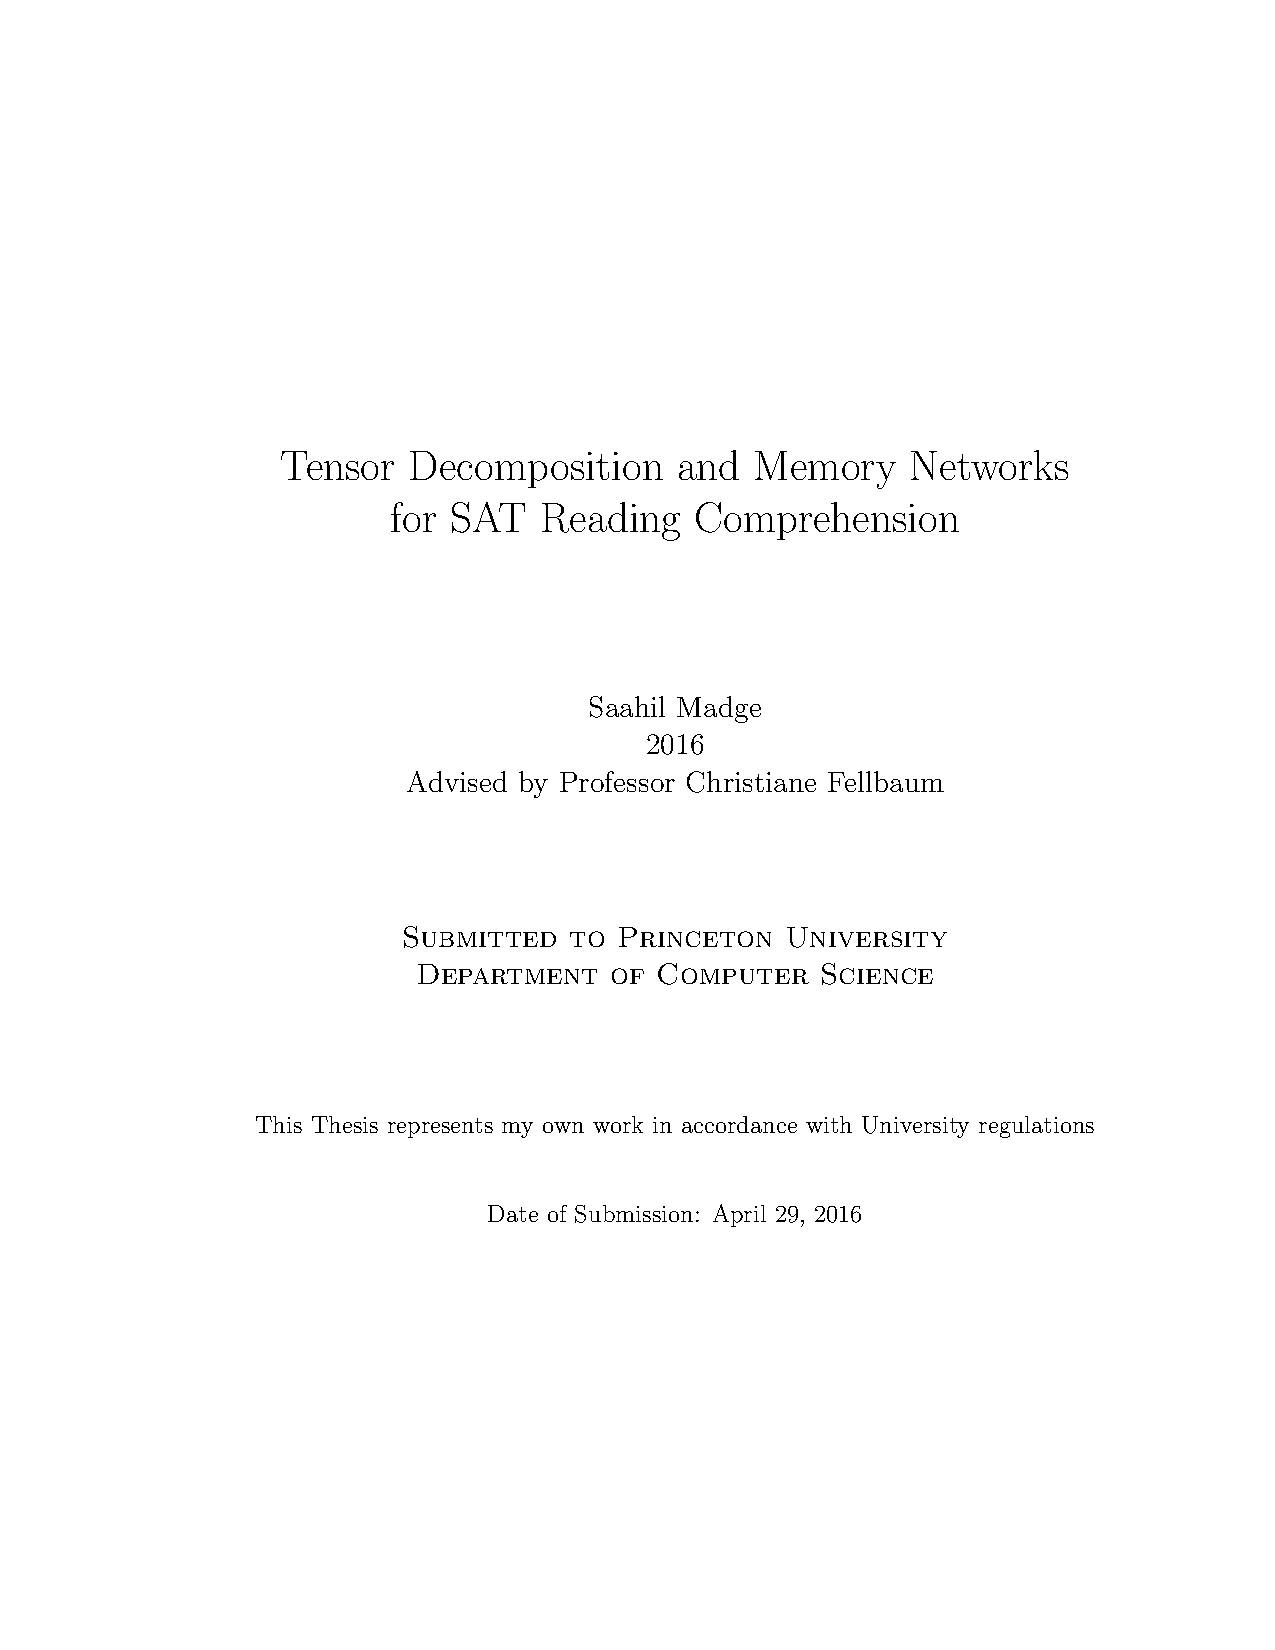
\includepdf{titlepage.pdf}

\newgeometry{left=1.5in, top=3in, right=1in}
\begin{abstract}

    \noindent We present a general approach for machine comprehension tasks by
    converting the text to a knowledge graph and the questions to queries on the
    graph. We extend \cite{Narasimhan2015} and use the Stanford NLP Toolkit's
    Dependency Parser \cite{Manning2014, Chen2014} to transform each sentence
    into a set of entity-relation triples. We use word2vec \cite{Mikolov2013} to
    convert the questions into queries on the graph. We present a tensor
    decomposition approach to answering queries by adding Semantically Smooth
    Embedding \cite{Guo2015} to RESCAL \cite{Nickel2011}. We also generalize the
    Memory Networks \cite{Weston2015a, Sukhbaatar2015} to take any knowledge
    graph as input. We evaluate these models on three full SAT reading
    comprehension tests. The models presented here perform better than their
    respective baselines. Both models demonstrate the ability to answer
    questions based on the semantic and structural information in the text.

\end{abstract}
\restoregeometry

\newpage

{\large \tableofcontents}
\newpage
% \title{
% Solving SAT Reading Comprehension Questions with Memory Networks}
%
% \author{Saahil Madge\\Advisor: Professor Christiane Fellbaum}
%
% \date{}
% \maketitle

\thispagestyle{empty}
\doublespacing
% \begin{abstract}
% This document is intended to serve as a sample you can use for independent work reports.  We provide some guidelines on content and formatting.  They are not required, but they might be helpful.
% \end{abstract}

\section{Background and Motivation}
\label{Background and Motivation}

Machine question-answering (QA) has been a popular subject in recent research.
It is a very interesting field from an academic perspective, requiring
knowledge and techniques across the areas of artificial intelligence, machine
learning, natural language processing, linguistics, and mathematics.

QA has applications to many aspects of daily life. A famous use of
question-answering techniques is in Apple's Siri program. Siri combines speech
recognition software with question-answering techniques to create a virtual
iPhone assistant. Another example is IBM's Watson, which answered questions in
many subjects and performed quite well as a contestant on the game show
\textit{Jeopardy!} A less spectacular but more commonly-used example can be seen
by typing in a simple question such as \textit{How many calories are in an
apple?} on Google. The search results provide a detailed nutritional breakdown
of an apple.

The general term QA covers a broad array of subfields. Information retrieval,
factual question-answering, reading comprehension, and inference are all part
of the greater question-answering area. QA is a rapidly evolving field, but as
the examples above indicate, recent research has focused extensively on
answering spoken questions, and factual questions.

However, the subfield of machine comprehension has not been studied nearly as
well, though it has become quite popular in the past few years. Machine
comprehension involves training programs and systems to read text and answer
questions based on the newly acquired information. In most other QA tasks, the
system has a large database of facts (knowledge base) and must interpret the
question and provide the relevant factual answer. Machine comprehension tasks,
on the other hand, require the system to parse both the informational text as
well as the question, and then provide the correct answer. As there is
possibility for error within the knowledge base, machine comprehension tasks
are some of the most difficult QA tasks.

Machine comprehension has a wide range of applications. Reading comprehension
tests are a natural choice, but fields like document retrieval also use machine
comprehension techniques. Financial firms that use news analysis to make
trading decisions heavily rely on these techniques as well. Many long-term
goals of AI such as dialogue and humanoid robots cannot be achieved without
significant advance in this area \cite{Weston2015}. Another incentive to
study machine comprehension is that new research here can be applied to drive
research in many other areas of artificial intelligence and natural language
processing.

As a consequence of machine comprehension tasks being so difficult, most
research with reading comprehension tests has focused on elementary school level
tests. The most common dataset is MCTest \cite{Richardson2013}, which we discuss
in more detail in Section \ref{Related Work}. This dataset is a set of passages
and reading comprehension questions created by crowdsourcing. The stories are
``carefully limited to those a young child would understand''
\cite{Richardson2013}. Another common dataset is Facebook's bAbi dataset
\cite{Weston2015}, which has a collection of short toy problems that can be used
to train machine comprehension systems. These problems could certainly be solved
by a human elementary school student. Berant et al. \cite{Berant2014} train a
system to answer questions based on a paragraph describing biological processes,
which is certainly an advanced topic, but the system is specialized for
biological tasks and not applicable as is to general reading comprehension.

In this paper we focus on SAT reading comprehension questions. The major reason
is that they are far more complex than MCTest questions and other commonly-used
machine comprehension datasets. The sentence structures, vocabulary, and topics
covered in SAT passages are all far more varied than in the other benchmarks.
The questions are much harder as well, and simply understanding the question and
the individual choices is difficult by itself. SAT questions often test
underlying themes and broad ideas rather than particular factual details
(``Why'' or ``How'' questions). In contrast, MCTest questions are often of a
``Who'', ``When'', or ``What'' form, which have traditionally been easier for
programs to answer.

Another aspect that makes SAT questions so difficult is that they require
inference to answer, as opposed to just matching words or syntax. MCTest and
similar questions can mostly be answered through word-matching (discussed in
Section \ref{Bag-of-words}) or via syntactic matching. Word-matching means the
system will try to find which sentences in the passage have the most words in
common with the query, and use that to choose an answer. Syntactic matching is
the same principle, but aims to match syntactic structure. SAT questions,
however, almost never repeat the answer words in the question itself, and the
query structure is not correlated with passage structure. To solve these
questions, our system has to really understand the high-level concepts and
information that is implied but not directly on the surface. This is a
significantly harder problem than has been tackled before, but it is necessary
to solve to continue moving forward in the field of machine comprehension. By
trying to answer SAT questions we can try to solve problems that will be present
in real-world applications but have not yet been tackled by existing research.

Due to the difficulty of interpreting the text as-is, we represent the text
using relational logic instead. We dynamically create a \textit{Knowledge Graph}
(covered in more detail in Section \ref{Representation Techniques}) as we parse
through the text and try to frame each question as a query on this knowledge
graph. The knowledge graph representation is typically used for factual data
that has already been collected in entity-relation triple form. As far as we
know, no previous research in this space has tried to dynamically create a
knowledge graph on which we can answer questions.

Traditionally most research on relational learning has used either neural
networks or tensor decomposition to answer queries on the graph. In this work we
present an improved version of both methods. For tensor factorization we enhance
a method known as RESCAL \cite{Bader2007, Nickel2011} with a technique known as
\textit{Semantically Smooth Embedding} \cite{Guo2015}. RESCAL trains a
factorization of the knowledge graph using Alternating Least Squares, and this
factorization can then be used to answer queries.

The neural network approaches such as TransE \cite{Bordes2013} and TransH
\cite{Wang2014} use neural networks to train an embedding method for the
relations on the knowledge graph, and use the trained model to answer queries.
However, none of these previous approaches are designed for question-answering.
We enhance the Memory Networks architecture proposed by Weston et al.
\cite{Weston2015a} and improved by Sukhbaatar et al. \cite{Sukhbaatar2015} to
take knowledge graph triples and queries as input, and provide a scoring of the
answer choices as output. We discuss memory networks and alternatives in much
greater depth in Section \ref{Related Work} and Section \ref{Model}.

All models and data are available at
\url{https://github.com/SaahilMadge/Senior-Thesis}. Our goal with this research
is to present a way to combine ideas that were previously used in isolation for
QA or other learning tasks into a system which can parse and interpret a complex
text, and answer difficult high-level questions about the text. The text,
questions, and techniques we use are more ambitious than those studied in
previous research. We hope that this paper will encourage others to tackle
problems of equal or greater ambition, and drive progress in the development of
safe artificial intelligence.

\section{Technical Review}
\label{Technical Review}

In this section we review some of the techniques that are used in previous
research and in this paper.

\subsection{Representation Techniques}
\label{Representation Techniques}

We begin by reviewing various methods for embedding text and performing queries
on the embedded representations.

\subsubsection{Bag-of-words}
\label{Bag-of-words}

Bag-of-words is a type of analysis in which we treat each sentence as simply a
collection of words, without paying attention to their order or the dependencies
between individual words. If we have some vocabulary of size $V$, we can encode
each sentence as a vector of size $V$ where each vector element corresponds to
some word in the vocabulary. If the word appears in the sentence we store how
many times it appears, and if it does not appear we store it as a 0. This is
known as \textit{one-hot} vector encoding. Most designs encode each input
sentence and the query as one-hot vectors. These vectors are not used as-is, but
are first embedded into some dimension $d$. The learning algorithm is run on the
embedded vectors, and we can output a response in a specified format. Two common
methods are to return a probability vector of size $V$ where each element
represents how likely that word is to be the output, or to pick the most likely
word from that distribution and return only that word.

\subsubsection{Dependency Parsing}
\label{Dependency Parsing}

Dependency parsing is an important technique used to understand the structural
information in a sentence. Essentially, dependency parsing creates a graph of
the words in the sentence and describes how each word relates to other words,
using the standard Universal Dependencies \cite{De2014}. A sample graph is shown
in Figure~\ref{fig: dependency parsing}, from \cite{Chen2014}. Each dependency
in the graph has a \textit{governor} and \textit{dependent}. The collection of
dependencies contains all the structural relationships in the sentence. Each
dependency is labelled to show the exact relationship between governor and
dependent. For example, in the graph in Figure~\ref{fig: dependency parsing} the
label \textit{nsubj} highlights the nominal subject of a particular clause in
the sentence \cite{De2014}. The specific parser we use is the Stanford
High-Performance Dependency Parser by Chen and Manning \cite{Chen2014}.

\begin{figure}[!tb]
    \centering
    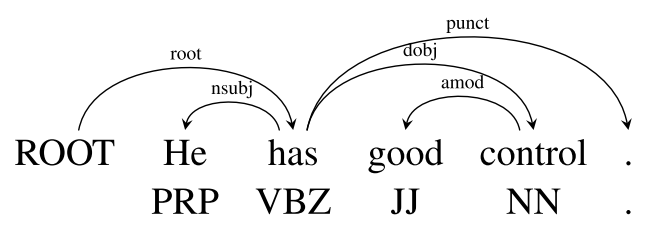
\includegraphics[width=0.7\textwidth,keepaspectratio]{figures/Dependency_Graph.png}
    \caption{A small example knowledge graph, from \cite{Chen2014}}
    \label{fig: dependency parsing}
\end{figure}

Once the dependency graph is created, we can analyze it to extract the relevant
information in the sentence. The exact details are discussed more in Section
\ref{Converting to Knowledge Graph Representation}. The basic approach is to
find the main subject of the sentence and either the direct object it acts on or
some description of it. Then it can be turned into an entity-relation triple on
the knowledge graph.

\subsubsection{word2vec}
\label{word2vec}

The \textit{word2vec} embedding technique introduced by Mikolov et al.
\cite{Mikolov2013} is perhaps the most common embedding technique used in NLP
research. It is actually an umbrella term for various methods, such as
\textit{skip-gram} or even bag-of-words embedding. The word2vec techinque
produces a vector representation of words, often with several hundred elements.
These representations can then be manipulated as vectors in the
higher-dimensional space, allowing for interesting operations on words. For
example, \textbf{vector(``king'')} - \textbf{vector(``man'')} +
\textbf{vector(``woman'')} produces a vector that is very close to
\textbf{vector(``queen'')}. The reason word2vec is able to embed so successfully
is generally thought to be the fact that the process of embedding gives similar
words a similar embedding (which is measured by cosine similarity). The cosine
similarity measure is also used to find the similarity between two arbitrary
words. $word2vec.similarity(\text{word1}, \text{word2})$ is a function within
word2vec which returns a measure between 0 (not at all similar) and 1
(identical).

\subsubsection{Knowledge Graph Overview}
\label{Knowledge Graph Overview}

A knowledge graph generally refers to a set of \textit{entity-relation triples}.
These triples take the form $\langle e_1, r, e_2 \rangle$. where $e_1$ and $e_2$
are entities and $r$ describes the relation between these two entities. Entities
and relations (collectively referred to as \textit{labels}) can be repeated
across triples. The total set of triples denotes all the knowledge in our
``Knowledge Base''.

\begin{figure}[!tb]
    \centering
    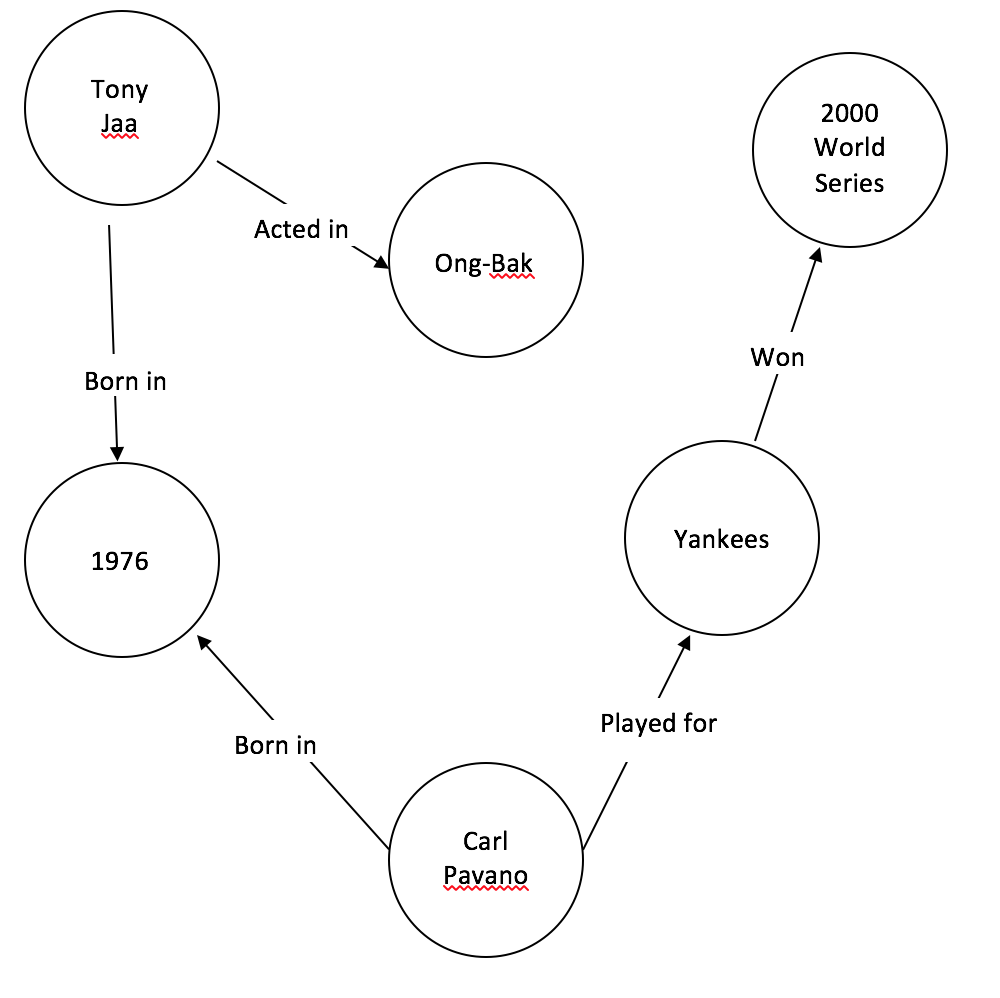
\includegraphics[width=0.7\textwidth,keepaspectratio]{figures/Example_KG.png}
    \caption{A small example knowledge graph}
    \label{fig: KG}
\end{figure}

We can represent these triples as a directed graph, with each entity as a vertex
and the relations as edge types between them. Figure \ref{fig: KG} shows an
example of a very small knowledge graph. Note that there is only one node per
entity. This allows the graph to store multiple pieces of information regarding
the same entity together, to allow for easy processing by the program while also
making it simple for humans to understand. The mathematical details of our
knowledge graph model can be found in Section \ref{Model}.

Once a knowledge graph is built, we can pose queries about the graph. For
example, we can provide two entities $e_1$, $e_2$ and ask which relation $r$
links the two on the graph. We can also provide an entity $e$ and the relation
$r$, and ask for which other entity $e'$ do the triples $\langle e,r,e' \rangle$
or $\langle e',r,e \rangle$ exist on the graph. Put another way, the queries are
either \textit{link prediction} queries or \textit{entity prediction} queries.

\subsection{Neural Networks}
\label{Neural Networks}

As discussed in Section \ref{Background and Motivation}, recent research in
machine comprehension has extensively used neural nets (NNs) and their variants.
Here we provide a quick review of neural network design. These topics can be
covered in far more depth in \cite{Bishop1995, Nielsen2015}.

\subsubsection{Feed-forward Neural Networks}
\label{Feed-forward Neural Networks}

The most basic model is known as a \textit{feed-forward} neural net. These have
several layers composed of units (nodes). There is an initial input layer, a
final output layer, and \textit{hidden layers} in the middle. A unit in layer
$l$ takes as input the output of nodes in the previous layer (or the actual
input if this is the input layer). It multiplies these by some weight matrix
$W^l$, transforms it using an activation function $g$, and sends its output to the
next layer (or as the final output if this is the output layer). Common
activation functions are the $tanh$ and $sigmoid$ functions. The sigmoid
function is defined as $\sigma (x) = \frac{1}{1+e^{-x}}$. For now we will assume
that our activation function is sigmoid.

Mathematically, we define the input to the current layer as $x^{l-1}$,
where $x^{l-1}_{ij}$ means that it is the input from unit $j$ in the previous
layer to unit $i$ in the current layer. $W^l_{ij}$ is the weight on this
connection, defined as 0 if node $i$ does not depend on node $j$. The output of
node $j$ is $\sigma ( W^l x^{l-1}_j)$. Typically the quantity $Wx^{l-1}_j$ is
known as $z_j$. We can also define bias vectors $b$ such that $z_j =
W^lx^{l-1}_j + b^l_j$. To summarize, we can write the output of some layer $l$
in vector notation as
$$o^l = \sigma(W^lx^{l-1} + b^l)$$

We can propagate this forward starting at the input layer, through the hidden
layers, and finally at our output layer. We can then train our network using the
backpropagation algorithm. We have some cost function $C$ that is a measure of
the error of our output. We find the error at the output layer, and then change
the weights at each previous layer, working backwards to the input layer. The
key to backpropagation relies on updating the weights based on their partial
derivatives with relation to $C$. In-depth derivations are provided in
\cite{Bishop1995, Nielsen2015}.\\

\subsubsection{Recurrent Neural Networks}
\label{Recurrent Neural Networks}

Feed-forward networks are good tools, but do not have any form of state
(memory). Here we review recurrent neural networks (RNNs) which have a hidden
state $h_t$.

At step $t$ in a recurrent neural network, we have input $x_t$ and a hidden
state $h_{t-1}$. We also have weight matrices $U$ and $W$. We can define the
current state $h_t = \sigma(Ux_t + Wh_{t-1})$. We have another weight matrix $V$
for the output. The output $y_t = softmax(h_t)$, where $softmax(z_i) =
\dfrac{e^{z_i}}{\sum_j e^{z_j}}$. The softmax function output is a probability
distribution over the vector.

Using the softmax function has several advantages. Because it is a smooth
function, we can take its derivative, making it easier to calculate the
backpropagation equations. Additionally, most RNNs and variants use a loss
function known as cross-entropy loss. If the model output is $\hat{y}$ and the
true output is $y$, then cross-entropy loss is defined as $C = -\sum_i y_i
\log(\hat{y_{i}})$. When we pair a softmax output with cross-entropy loss, the
error at the output node $i$ is simply $\hat{y_i} - y_i$. This is very
convenient because it can be calculated rapidly, so it allows for fast training
of the RNN. Training is normally a bottleneck, and by combining a robust output
function and robust loss function we get a very elegant output error. As this is
a very important result, we have included it in Section \ref{Derivation of
Output Layer Error}.

\section{Related Work}
\label{Related Work}

The first major research in machine comprehension was conducted by Hirschman, et
al. \cite{Hirschman1999}. Their system ``Deep Read'' takes a story and a series
of questions as input, and proposes answers by using bag-of-words techniques
with other methods such as stemming and pronoun resolution layered on top. On a
collection of remedial reading questions for grades 3-6, Deep Read answered
about 40\% of the questions correctly.

Most recent research has used the MCTest \cite{Richardson2013}, released by
Richardson, et al. at Microsoft research. There are a total of 500 passages,
each with 400 questions, created at the reading level of a young child. The
stories are fictitious, which means the answers can only be found in the story
itself. Richardson et al. also provide two baseline implementations to serve as
a benchmark. The first is a simple bag-of-words model with a sliding window. It
scores about 51\% accuracy on the MC500 questions. The second implementation
adds a distance-based scoring metric and reaches 56\% accuracy. Both
implementations score significantly higher on questions where the answer is
contained in just one sentence than on questions where the answer requires
information across multiple sentences.

Narasimhan and Barzilay \cite{Narasimhan2015} also work on the MCTest tasks.
Their main insight is to create a task-specific discourse parser to capture
specific discourse relations in the MCTest passages, while the prevailing method
had been to use generalized off-the-shelf discourse parsers. They create three
models of increasing complexity. The first assumes each question can be answered
using just one sentence, and estimates a joint probability distribution across
the question, query, and answer. The second model adds in the joint distribution
across a second sentence as well, to handle the case in which the answer needs
two sentences to answer. The third model incorporates discourse relations
between the two sentences to better understand the relationship between
information in each sentence. The relations are defined as ``Causal'',
``Temporal'', ``Explanation'', and ``Other''. Most systems have performed the
worst on these types of questions. By focusing specifically on modeling these
explanatory relations, the third model easily outscores the other two, and the
two MCTest baseline implementations, achieving almost 64\% accuracy.

Berant et al. \cite{Berant2014} also focus on analyzing inter-sentence
relations, with application specifically to passages and questions about
biological processes. These passages generally describe a chemical reaction or
other process in which there are various starting entities which interact with
each other and form a new output. Understanding how the inputs interact and
tracing the flow of the process is crucial to answering the question. To solve
this, Berant et al. define events (or non-events) as ``triggers'', and try to
find relationships between events. The events can be thought of as nodes on a
graph, with an edge defining some relation between the two. There are eight
possible relations, including ``cause'', ``enable'', and ``prevent''. They first
create events and then predict relations between the events. The queries are
also formulated as a graph. They are categorized as dependency questions,
temporal questions, or true-false questions. This model scores almost 67\% on
the dataset, over 6\% better than the next-best model.

Most recent machine comprehension research has focused on using neural nets as
the core system. Neural nets are a very generalizable technique and in the past
decade have become very popular. In fact, advances in neural net techniques have
greatly contributed to the recent surge in machine comprehension research.

Weston et al. \cite{Weston2015a} introduced memory networks. These are a type of
neural network which simulate a long-term memory. We discussed in Section
\ref{Recurrent Neural Networks} how RNNs have a ``vanishing gradient'' problem,
and are not able to take advantage of states from more than a few steps prior.
Memory networks have a memory module which stores old memories and then updates
them given new inputs. When given a query, the memory network finds relevant
memories, then finds memories that are relevant given those memories, and so on.
Finally, it provides an answer to the query. Sukhbaatar et al.
\cite{Sukhbaatar2015} improved this model by creating a model that can be
trained end to end, while in the original design each module needed to be
trained independently. This is the model that is the basis for our design, so we
discuss it in more detail in Section \ref{Model}. Kumar et al. \cite{Kumar2015}
create ``Dynamic Memory Networks''. Their design uses two memory modules. The
semantic memory module stores general knowledge, while the episodic memory
module iteratively finds memories relevant to the query.

Knowledge Graphs are also a popular research area. There are two main approaches
that are used for solving knowledge graph embedding and query problems. The
first is the neural network embedding style, popularized by Bordes et al.
\cite{Bordes2013} and improved by Wang et al. \cite{Wang2014}. Bordes' TransE
and Wang's TransH both train a neural network to recognize triple embeddings in
some higher dimension. The triples are embedded in such a way that triples that
are ``similar'' according to some metric are embedded near each other. Queries
can be answered more easily using the embedded vectors.

The second approach focuses on representing the knowledge graph as a tensor.
Nickel et al. \cite{Nickel2011} proposed RESCAL, a model which converts the
knowledge graph into a tensor of adjacency matrices and trains a latent rank-$r$
factorization of the tensor using a technique called ASALSAN \cite{Bader2007}.
Queries about the knowledge graph can be easily converted into searching over a
relevant subset of elements in the factorization. Chang et al. \cite{Chang2014}
created TRESCAL, which is an optimized version of RESCAL.

\section{Model}
\label{Model}

This research presents three fundamental insights. \\

\begin{enumerate}

    \item We treat the input text as a knowledge base and dynamically convert it
    into a knowledge graph. We can then interpret the questions as queries on
    the graph, requiring us to find an entity or relation that represents the
    answer to the question. \\

    \item We use tensor decomposition to embed the knowledge graph and
    questions. Specifically, we use an enhanced version of RESCAL
    \cite{Nickel2011}. RESCAL by itself is a fine model, but we make it more
    accurate by adding ``Semantically Smooth Embedding''(SSE), as proposed by
    Guo et al. \cite{Guo2015}. In their original paper they propose adding this
    type of embedding to tensor decomposition as future work, so to our
    knowledge we are the first to perform tensor decomposition with SSE. \\

    \item We embed the knowledge graph and questions into input vectors, and
    pass them into a Memory Network. Given a set of embedded inputs and queries,
    this type of neural network takes advantage of ``memory'' to find new facts
    that are relevant given the current set of relevant facts, but may not be
    relevant solely based on the query. \\

\end{enumerate}

These techniques were first introduced in previous research. However, all of
them were applied to separate domains. Neural nets have been used for machine
comprehension on MCTest, bAbi, and questions of similar difficulty. Their
embedding model is quite simple, however (often just bag-of-words). Knowledge
graphs and tensor decomposition have traditionally been used only for relational
learning when a knowledge graph or set of triples already exists. As our problem
is more complex than that tackled by these original models, and we must combine
these original models, we have to significantly modify their conceptual and
mathematical basis.

\subsection{Knowledge Graph Representation}
\label{Knowledge Graph Representation}

The first part of our design is to dynamically convert the input passage into a
knowledge graph and the questions as queries on that graph. \\

\subsubsection{Advantages of Knowledge Graph Representation}
\label{Advantages of Knowledge Graph Representation}

There are several advantages to using a knowledge graph representation. The main
benefit is that it actually preserves the meaning of the text. Whereas
bag-of-words loses the semantic and structural information in a sentence, a
knowledge graph representation almost completely stores the intended meaning of
the original text. Most sentences in English can be broken down into
Subject-Verb-Object triples, which require little if any processing to convert
into the $\langle \textit{entity}_1, \, \textit{relation}, \, \textit{entity}_2
\rangle$ format. The knowledge graph itself is simply a list of these triples.
If we can parse the input text and extract the Subject-Verb-Object relationship,
we can convert each sentence into a triple of the form
$$\langle \textit{subject}, \, \textit{verb}, \, \textit{object} \rangle
\Rightarrow \langle e_1, \, r, \, e_2 \rangle$$
The details of the conversion are covered in Section \ref{Converting to
Knowledge Graph Representation}.

Even more importantly, the knowledge graph inherently has \textit{memory}. What
this means is that it automatically pieces together information about the same
concept, even if that information occurs across different sentences or even
different paragraphs. Consider a passage about a boy named Harry. Even if in one
paragraph the text says that Harry was born in 1980 and several paragraphs later
we learn that he has a friend named Ron, these relations both link to the single
Harry entity node. By analyzing the outbound and inbound relations of the Harry
entity node, we can easily find all the information the text has stated about
Harry. Any question asked about Harry can be answered using this information.
While such a representation for memory may seem natural, virtually all previous
research in the machine comprehension space has parsed by sentence. As a result,
the knowledge graph representation is the best way for our system to easily find
all information about an entity that was given in the original text.

Entities also do not have to be concrete things; they can just as easily be
abstract concepts. For example, Figure~\ref{fig: KG} shows entities like Carl
Pavano (a person), but it also shows an entity node for the year 1976. To
roughly generalize, any noun can be an entity node. The phrase ``abstract
concept'' itself could be an entity node. Entity-relation triples can all be
analyzed similarly, so abstract reasoning is as simple as concrete reasoning.
Not only does a knowledge graph allow us to perform abstract reasoning, but it
is arguably the only way to perform reasoning of this form.

A good way to understand the knowledge graph representation is to think of it as
a \textit{concept map}. Every sentence in the text introduces a new concept
(concrete or abstract) and/or provides more information about a previously
introduced concept. All information is provided in such a way that the concept
is either the actor or the receiver of some action. We update our concept map
with this new information by adding entity nodes as needed and the relation
provided in the current sentence. When we've finished parsing the input text,
we have the full concept map, which gives complete information on each concept
and the information we know about it.

Another benefit is that there are already methods and theory of analysis for
knowledge graphs. As mentioned earlier, passages as complex as SAT reading
comprehension tests have rarely been analyzed semantically. Moreover, the fact
that information comes in a variety of sentence structures across several
paragraphs means that traditional semantic analysis will not suffice.
Traditional analysis often parses one sentence or one paragraph at a time, which
is not enough for our particular use case. The original input simply cannot be
analyzed as it is using existing techniques. Since this problem cannot be solved
in its original form, we convert it to a form which we know how to analyze. Not
only have knowledge graphs been studied extensively in the field of relational
learning, but they can also be analyzed using techniques from graph theory.
Essentially, we turn the problem of analyzing complex text into a problem of
analyzing a knowledge graph.

At the same time, the knowledge graph representation also preserves human
readability. A major problem with text input is that it is easily interpretable
by humans but requires much preprocessing before it can be interpreted by a
program. It is not necessary for our processed text to be in a format humans can
interpret, but it certainly helps us reason about the problem and come up with
interesting solutions. The entity-relation triple format is almost as intuitive
to humans as the original textual input.

Of course, even the knowledge graph representation has some drawbacks. Because
we build the knowledge graph using the statements in the original text, we can
only perform analysis on the textual information. We can trace relations through
the graph but there is no way to perform higher-level reasoning. For example,
questions that ask about classification of new information or broad themes of
the passage cannot be answered. Nevertheless, these are flaws in any form of
representation. The knowledge graph representation provides the most advantages
and fewest drawbacks of any representation. \\

\subsubsection{Converting to Knowledge Graph Representation}
\label{Converting to Knowledge Graph Representation}

In this section we present the exact details of converting the text into a
Knowledge Graph. Section~\ref{Data} discusses how the raw tests are converted
into textual information that we can then parse.

We use the Stanford High Performance Dependency Parser \cite{Chen2014} to
extract the entity-relation information from the text. Section \ref{Dependency
Parsing} explains how this tool creates a dependency graph of a particular
sentence. We then provide a set of semantic rules to isolate the important
information and create a triple from it. Figure~\ref{fig: dependency extraction}
from \cite{Narasimhan2015} shows a simple sentence, as well as the extracted
triple.

\begin{figure}[!tb]
    \centering
    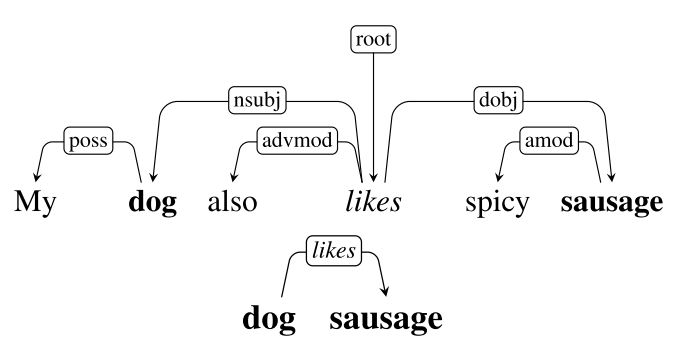
\includegraphics[width=0.7\textwidth,keepaspectratio]{figures/Dependency_Extraction.png}
    \caption{Extracting an entity-relation triple from a sentence, from \cite{Narasimhan2015}}
    \label{fig: dependency extraction}
\end{figure}

The information extracted should conform to knowledge graph format, namely
\\$\langle \text{entity}_1, \,\text{relation}, \,\text{entity}_2 \rangle$. We
want to frame the information in the sentence so that it is one entity with some
relation to another entity. Most sentences are of the form where the subject
performs some action or has some description, so we focus on these two types of
sentences. In each sentence we isolate the main subject using the \textit{nsubj}
dependency. Then we check for one of two relations. If the subject is performing
some action then the sentence can be generally extracted as $\langle
\text{subject}, \,\text{action}, \,\text{direct object} \rangle$. In this case
the \textit{dobj} dependency is used to extract the action verb as well as the
direct object. Figure~\ref{fig: dependency extraction} shows this case. In the
second case, the sentence is often of the form ``<subject> is...
<description>''. Here we use the \textit{cop} dependency to extract the verb and
the description. The triple $\langle \text{subject}, \,\text{copular verb},
\,\text{description} \rangle$ is added to the knowledge graph. In English,
``verbs of being'' such as ``is'', ``are'', ``were'', etc. are all copular
verbs. Narasimhan and Barzilay \cite{Narasimhan2015} do a similar type of
extraction, but they create what they call an \textit{entity graph}, which is
slightly different from our knowledge graph. Their entity graph refers to
linguistic entities from the dependency parsing, while our knowledge graph
refers to information, not linguistic objects.

\subsection{Tensor Decomposition}
\label{Tensor Decomposition}

First we discuss the tensor decomposition approach to answering SAT questions.
The advantage of using tensor decomposition is that it is based on
well-understood mathematics, rather than simply empirical validation as with the
neural network.

Our model is an improved version of RESCAL, proposed by Nickel et al.
\cite{Nickel2011} and used by Chang et al. \cite{Chang2014}. RESCAL itself takes
the general tensor decomposition model proposed by Bader et al. \cite{Bader2007}
and modifies it to work for relational learning. \\

\subsubsection{Knowledge Base Tensor}
\label{Knowledge Base Tensor}

The tensor decomposition approach treats the knowledge graph as a directed
graph. A tensor is simply a multi-dimensional array. In our case, we use a
three-dimensional array $\mathcal{X}$ to represent the knowledge graph. If we
have $N$ entities $e_1, e_2, ..., e_N$ and $M$ relations $k_1, k_2, ..., k_M$
then we can consider $\mathcal{X}$ as $M$ layers of $N\times N$ matrices. Each
layer $\mathcal{X}_k$ tells which entities are linked by relation $k$. If we
denote our knowledge base as $KB$, then $\mathcal{X}$ is formulated as

$$
\mathcal{X}_{ijk} =
\begin{cases}
    1 & \text{if } \langle e_i,\,k,\,e_j\rangle \in KB \\
    0 & \text{otherwise}
\end{cases}
$$

\begin{figure}[!tb]
    \centering
    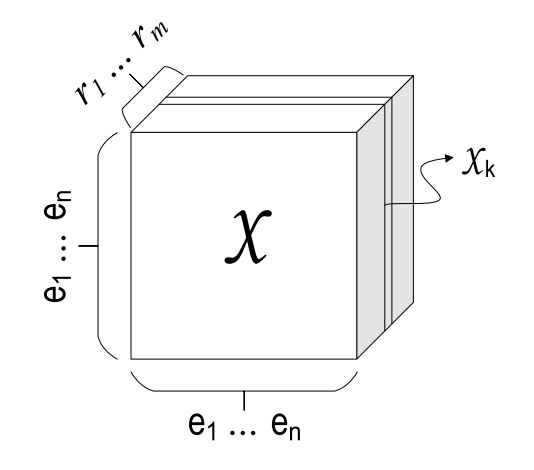
\includegraphics[width=0.7\textwidth,keepaspectratio]{figures/tensor_figure.png}
    \caption{A graphical representation of $\mathcal{X}$, from \cite{Chang2014}}
    \label{fig: tensor figure}
\end{figure}

Figure~\ref{fig: tensor figure} from \cite{Chang2014} presents a graphical view
of $\mathcal{X}$. $\mathcal{X}$ is essentially a series of adjacency matrices
$\mathcal{X}_k$, where each matrix only marks edges of relation type $k$. \\

\subsubsection{Tensor Factorization Overview}
\label{Tensor Factorization Overview}

Our approach aims to factorize the tensor and take advantage of the inherent
structure of the graph. To that end we train a rank-$r$ factorization of each
slice, as suggested in \cite{Bader2007, Nickel2011}.

$$X_k \approx A R_k A^T \text{ for } k \in [1,m]$$

Here, A is an $n\times r$ matrix which contains the latent-component
representation of the entities in the knowledge graph. We can think of this as
an $r$-dimensional embedding of the entities, where each entity has $r$ hidden
features. This is conceptually similar to the word2vec embedding, where each
feature of a word vector does not necessarily mean something intuitive but is a
hidden component found through training.

$R_k$ is an $r\times r$ matrix which represents how these hidden features
interact with each other for the $k$-th relation. $R_k$ is asymmetric, which
means that the hidden feature interactions are one-way. It is not necessarily
true that $R_{ijk} = R_{jik}$, although it could be. Note that $R$ itself is
also a three-dimensional tensor of shape $r\times r\times k$.

We decompose the tensor so that we can answer queries using the factorization,
which has the hidden components of the graph and is thus more generalizable, as
opposed to using the original tensor which is simply an adjacency tensor of the
knowledge graph. A particular connection between two entities, for example,
might not be explicit on the knowledge graph but can be uncovered by the
factorization.

We frame the problem of finding $A$ and $R_k$ as an optimization problem, where
we aim to minimize the difference between the original matrix $\mathcal{X}_k$
and its factorization $AR_kA^T$. Specifically, define the loss function $f$ as
the squared frobenius norm of this difference.

\begin{equation}
\label{eq: loss function}
    f(A, R_k) = \dfrac{1}{2} \sum_k \norm{\mathcal{X}_k - AR_kA^T}_F^2
\end{equation}

where the frobenius norm of some $a\times b$ matrix X is defined as

$$\norm{X}_F = \sqrt{\sum_{i=1}^a \sum_{j=1}^b |X_{ij}|^2}$$

To find the optimal $A$ and $R_k$, we just have to minimize Equation~\eqref{eq: loss
function}, along with some regularization function $g(A, R_k)$. Formally,

\begin{equation}
    \label{eq: to minimize}
    \underset{A, R_k}{\text{min }} f(A,R_k) + \lambda g(A, R_k)
\end{equation}

In \cite{Nickel2011}\cite{Chang2014} the regularization term is simply defined
as $g(A, R_k) = \dfrac{1}{2}\lambda \left(\norm{A}_F + \sum_k \norm{R_k}_F\right)$. This is
a standard regularization function where $\lambda$ is a hyperparameter. The aim
is to prevent overfitting when we try to solve the optimization problem. We
enhance their approach by using a stronger regularization function which adds
more constraints on the factorization. \\

\subsubsection{Semantically Smooth Embedding}
\label{Semantically Smooth Embedding}

Semantically Smooth Embedding (SSE) was proposed by Guo et al. \cite{Guo2015} as
a way to improve the TransE \cite{Bordes2013} embedding model. Whereas the
traditional models embed each individual fact in isolation, SSE imposes
geometric constraints on the whole model.

Specifically, we modify the \textit{Locally Linear Embedding} (LLE) constraint.
This constraint states that each node should be roughly a linear combination of
its neighbors \cite{Roweis2000}. Guo et al. \cite{Guo2015} created a version
meant for neural net embeddings such as TransE, but is not applicable to the
tensor decomposition method. Here we review their version first and then present
our new version for tensor decomposition.

In the original implementation each entity was labeled with a category and
then embedded into a vector representation. All nodes in the same category as
$e_i$ were defined as its neighbors and this set was denoted $\mathcal{N}(e_i)$.
Then they defined

$$
w_{ij} =
\begin{cases}
    1 & \text{if } e_j \in \mathcal{N}(e_i) \\
    0 & \text{otherwise}
\end{cases}
$$

$$R = \mathlarger{\sum_{i=1}^n} \norm{\mathbf{e_i} - \sum_{e_j \in \mathcal{N}(e_i)} w_{ij}
\mathbf{e_j}}_2^2$$

where $R$ is the regularization term added to the loss function. The logic here
is that we suffer more penalty in our loss function when entities that are close
to each other in the original set (i.e. are neighbors) have embedded vectors
that are far from each other. We cannot use this equation for our purposes since
our entities do not have categories and we do not have embedded vectors, but we
can apply similar logic.

We propose defining the neighbor set of each entity $e_i$ in our graph as all
other entities for which there is a directed edge from $e_i$ to $e_j$ in the
knowledge graph. The full neighbor set matrix is denoted $W$.

\begin{equation}
    \label{eq: new wij}
    w_{ij} =
    \begin{cases}
        1, & \sum_k \mathcal{X}_{ijk} \geq 1 \\
        0, & \text{otherwise} \\
    \end{cases}
\end{equation}

\begin{equation}
    \label{eq: new neighbor set}
    e_j \in \mathcal{N}(e_i) \text{ iff } w_{ij} = 1
\end{equation}

That is to say, $w_{ij} = 1$ if and only if we have some relation $r$ for which
the triple $\langle e_i,\,r,\,e_j \rangle$ exists in the knowledge base. We do
not consider entities which are related to $e_i$ in such a way that $e_i$ is the
recipient of the relation. Note that this means the neighbor relation goes one
way. $e_j \in \mathcal{N}(e_i)$ does not imply that $e_i \in \mathcal{N}(e_j)$.

Now consider the nodes in $\mathcal{N}(e_i)$. Since $e_i$ is related to all of
these, and because we want to enforce some geometric structure on our
representation (as done by Guo) we claim that the latent properties of each node
$e_i$, as provided in the matrix $A$, should be some linear combination of its
neighbor set.

$$ A_i \approx \sum_{i=1}^n w_{ij}A_j = \sum_{i=1} W_iA$$

We can penalize more for an $A$ in which this distance is large. The reason we
made the neighbor relation only one way is that we do not expect a large number
of disconnected components of our knowledge graph, and a two-way neighbor set
would push every node to have the same latent representation. \\

\subsubsection{Solving the Optimization Problem}
\label{Solving the Optimization Problem}

The new, semantically smooth regularization function is

\begin{equation}
    \label{eq: new g}
    g(A, R_k) = \sum_{i=1}^n \norm{A_i - \sum_{j=1}^n w_{ij}A_j}_F^2 =
    \sum_{i=1}^n \norm{A_i - W_iA}_F^2
\end{equation}

We are now ready to actually solve for $A$ and $R_k$. We want to minimize $f(A,
R_k) + g(A, R_k)$. This is a nonlinear, non-convex optimization problem which
would require complicated techniques. Calculating $f$ and $g$ is expensive, so
we use the Alternating Least Squares(ALS) method \cite{Koren2009}. Specifically,
we use the ASALSAN factorization method \cite{Bader2007}.

ALS turns the non-convex optimization problem into a convex problem by fixing
one of the unknowns. Then the problem can be solved with ordinary least-squares
optimization, so we use the normal method of least-squares to update the unknown
variable. Then we alternate by fixing this unknown and changing the other
variable. The ordinary least-squares can be solved relatively fast (although
calculating inverse matrices is expensive) and since each unknown is calculated
independently (keeping the other fixed), the ALS algorithm can be easily
parallelized. These two aspects make it very computationally fast, a quality
necessary for our purposes.

We have

$$\bar{\mathcal{X}} = A\bar{R}(\mathbf{I}_{2m} \otimes A^T)$$

where $\otimes$ is the Kronecker product and

$$\bar{\mathcal{X}} = \left( \mathcal{X}_1\mathcal{X}_1^T ... \mathcal{X}_m\mathcal{X}_m^T \right)$$
$$\bar{R} = \left( R_1 R_1^T ... R_mR_m^T \right)$$

Then by ASALSAN we derive the following update rules. We first update $A$ while
keeping $R_k$ fixed.

$$A \leftarrow \bigg[ \sum_k \mathcal{X}_kAR_k^T + \mathcal{X}_k^TAR_k \bigg] \bigg[ B_k + C_k \bigg]^{-1}$$
where
$$B_k = R_k A^T AR_k^T,\,\,\,\,\,\,\, C_k = R_k^TA^TAR_k$$

To update $R_k$, we first fix $A$. Then we notice that if we vectorize
$\mathcal{X}$ and $R_k$, we can rewrite Equation~\eqref{eq: to minimize} as

$$f(R_k) = \norm{\textbf{vec}\left(\mathcal{X}_k\right) - \left(A \otimes A \right)
\textbf{vec}\left(R_k\right)}$$

where we have removed an extra term $\lambda \norm{\textbf{vec}(R_k)}$ because
$R_k$ is no longer in our regularization term. This rewritten $f$ is actually
a linear regression problem whose solution is

$$R_k \leftarrow \left( \left(A \otimes A \right)^T \left(A \otimes A\right)
 \right) ^{-1} \left(A \otimes A\right) \textbf{vec}\left(\mathcal{X}_k\right)$$

We alternate updating $A$ and $R_k$ until we have performed some maximum number
of iterations or until $\frac{f(A, R_k)}{\norm{\mathcal{X}_k}_F^2}$ is below
some tolerance $\epsilon$. The final factorization $\hat{\mathcal{X}}$ can now
be used to answer queries.

\subsubsection{Answering Queries}
\label{Answering Queries}

The first step in answering SAT questions with tensor decomposition is to
convert them to queries on the knowledge graph. Queries are either link
prediction queries or entity prediction queries (Section \ref{Knowledge Graph
Overview}). We use \textit{word2vec} to perform the conversion. As each entity
and relation is a word, we test the similarity of every word in the question to
every entity and relation. The two highest scoring graph labels (at least one
entity) are the knowns in our query. If there are two entities, then we have a
link prediction query. If there is an entity and a relation, then we have an
entity prediction query. The advantage of using word2vec similarity is that SAT
questions often rephrase the textual words. For example, if in the passage a
character is ``angry'', the question will use a word such as ``incensed'', which
does not exist in the knowledge graph, instead. word2vec translates unseen words
into  knowledge graph labels which can then be operated on.

Link-prediction queries are relatively simple to answer. Given $e_i, e_j$ we
return the relation $k$ that satisfies $\argmax{k}\,\, \hat{\mathcal{X}}_{ijk}$.
This is the relation which our factorization guesses is strongest between the
two entities.

Entity prediction queries are answered similarly. Given $e_i, k$ we return the
entity $e_j$ that satisfies $\argmax{j}\,\, \hat{\mathcal{X}}_{ijk}$. This is
the entity which our factorization guesses is most likely to be the recipient of
relation $k$ from entity $e_i$.

Once we find the label that satisfies the query, we test the similarity of this
label to every word in every answer choice, and pick the answer choice that
matches best. To summarize, we first convert the question a query on the
knowledge graph, find the label in the knowledge graph that answers the query,
and choose the answer that is most similar to it.

\subsection{Memory Networks}
\label{Memory Networks}

The second way we propose answering queries is with neural networks.
Specifically, an enhanced version of Memory Networks. The advantage of the
neural network approach is that it is very intuitive, computationally feasible,
and empirically proven. However, it does lack the strong theory of the
mathematical approach. We choose the Memory Networks architecture as the basis
for our model because it has strong performance on the bAbi dataset and the
foundational architecture itself scales easily to more complex problems as long
as the input is in a valid format. First we review the architecture as proposed
in \cite{Sukhbaatar2015}. Then we discuss how to adapt it to this specific
problem. \\

\subsubsection{Memory Network Architecture}
\label{Memory Network Architecture}

First we will review the architecture for one layer, as the extension to several
layers is straightforward. The basic model takes in a set of input vectors $x_1, ...,
x_n$ and a query vector $q$, and outputs an answer $a$. Memory Networks require
the input text and the query to be vectorized in some form for easy computation.
These embedding techniques are covered in detail in Section \ref{Representation
Techniques}. Typically the embedding is done with bag-of-words embedding. This
embedding technique relies on the same word being used in the answer choices as
well as in the original text, which is true for MCTest and bAbi. The vocabulary
comes from a dictionary of fixed size $V$.

The input vectors are converted into a set of memory vectors ${m_i}$ using a
matrix $A$ of size $d\times V$, where $d$ is a pre-determined dimension. $q$ is
also embedded into a state $u$ using a different matrix $B$ of size $d\times V$.
To find which memory vectors are most relevant to the initial query, we take the
dot product of each vector with $u$.

$$p_i = \text{Softmax}(u^Tm_i)$$

Since the softmax function returns a value between 0 and 1, each score $p_i$ is
a scalar that can be considered a probability of how relevant each memory vector
is to the query. The more relevant it is, the more likely it will help find the
answer.

The input vectors are now sent through another matrix $C$ to produce a set of
transformed inputs ${c_i}$. Each transformed vector $c_i$ is weighted by its
probability $c_i$ and the sum is taken as the output $o$ of that layer.

$$o = \sum_i p_i c_i$$

This output can then be fed as an input to the next layer, but in the single
layer case it is added to $u$ and sent through one final matrix $W$ of size
$V\times d$. Lastly, a softmax is taken on the result to yield a probability
distribution over the vocabulary space. This is designed to pick one word
or set of words as the answer.

$$\hat{a} = \text{Softmax}\left(W\left(o + u\right)\right)$$

The network itself is trained using backpropagation. The answers to the training
set questions are provided as input, and the network learns to answer them. The
exact details of training are covered in Section \ref{Evaluation Process}.

Several strategies can be used to extend the Memory Network to multiple layers.
We use the \textit{Recurrent Neural Network} strategy as it makes most sense for
our purposes. This strategy is the simplest to understand as well as to train.
Each layer acts the same as in the one-layer case. The only difference is that
for all layers $k > 1$ the input $u^{k+1} = u^k + o^k$, and the matrix $W$ is
only applied to $o^{final}$. Each layer uses the same $A,B,C$ matrices. By using
the same matrices at each level and passing the state along, this architecture
acts like a Recurrent Neural Network.

The initial layer calculates how relevant each memory vector is to the initial
query. That output is combined with the initial query and passed as $u$ to the
next layer. That layer finds how relevant each memory vector is to the new state
$u$. This means that memories which were not very relevant to the initial query
may be relevant to the memories which were relevant to the initial query. Each
layer finds new memories that can help answer the question. \\

\subsubsection{Memory Network Enhancements}
\label{Memory Network Enhancements}

As discussed, the original Memory Networks model uses simple bag-of-words
embedding to vectorize the text into the input vectors ${x_i}$. The problem with
this method is that the ``most relevant'' memories found in each layer are
relevant based on the exact word choice, not based on conceptual similarity. To
answer SAT questions the text must be vectorized in such a way that the
knowledge graph relationships are captured, and the question must be converted
into a query vector for the network. We need to change the inputs while
preserving the overall architecture so that the memories chosen as relevant
actually match the concept in the query, as opposed to simply matching the
words.

We propose stacking horizontally each slice of the tensor $\mathcal{X}$ as
defined in Section \ref{Knowledge Base Tensor} and using each column as an input
vector. In total the input matrix $\mathcal{X}'$ will be of shape $n\times
(nm)$. The query is more complicated to vectorize. The memory network
architecture requires the query to be a 1-dimensional vector. We create a vector
$q$ of length $N+M$ where $N$ is the number of entities and $M$ the number of
relations, where each element is 0. We find the two most similar labels as in
Section \ref{Answering Queries} and set their corresponding vector elements to
1. This is a two-hot encoding vectorization.

We make two changes to the original network architecture. We set the current
layer $u^k = R(u^{k-1} + o^{k-1})$, and $o$ is now the dot product of $Cx_i$ and
the $p_i$ vector, instead of being a scaled sum. Adding another matrix $R$
allows us to capture extra complexity across layers while preserving
dimensionality. Changing $o$ to be a dot product is also to help with
dimensionality. The original matrix had a fixed query size as well as input
length of 177, but with SAT questions the length $N+R$ is different for every
knowledge graph input, so we need to add more flexibility in the architecture
for this changing dimensionality.

The architecture equations become

$$m_i = Ax_i$$
$$u^0 = Bq,\, u^{k+1} = R(u^k + o^k)$$
$$p_i = \text{Softmax}\left(\left(u^k\right)^Tm_i\right)$$
$$c_i = Cx_i$$
$$o^k = \sum_i p_ic_i$$
$$\hat{a} = \text{Softmax}\left(W\left(o^l+u^l\right)\right)$$

where $l$ is the total number of layers.

In the multiple-layer case, the approach is the same as in the original model
where the matrix $C$ stays constant at each layer, and $u^{k+1} = u^k + o^k$.
Specifically we use a 10-layer neural network. The original paper used a 3-layer
model to find 3 steps of relevant facts. SAT questions require information
pieced together from many sentences, however, so we add more layers to capture
this additional complexity.

\subsection{Model Comparison}
\label{Model Comparison}

The Tensor model and the Memory Network model have the same underlying goal but
go about it very differently. Both models try to find the inherent properties
of the knowledge graph given the graph itself. Essentially, by finding this
latent representation of the graph, both models can answer questions about it.

The tensor model has a much stronger mathematical base. The RESCAL model uses
ASALSAN \cite{Bader2007} which is a general mathematical model for tensor
evaluation. Using ALS to optimize is an approximation to make the problem
computationally feasible, but the technique is still mathematically sound. At
the same time however, the tensor model is trained only on the knowledge graph
itself and not on the answers. IT is heavily reliant on the thoroughness of the
knowledge graph triples extracted from the text. Information that is missed in
the triple extraction will be lost to the tensor model as well.

The Memory Networks model is the exact opposite. It has a much weaker
theoretical base but is also more robust to errors in the knowledge graph
extraction process. The mathematics of neural networks are not as well
understood as that of tensors, especially as we add more layers. This means that
the neural net model we are using can behave in various unexpected ways.
Nevertheless, the model is trained using the answers to the training set
questions. It can find patterns and information using the training process, and
as a result is less subject to fluctuations in the actual knowledge graph
extraction.

\section{Data}
\label{Data}

The model evaluation is conducted on SAT tests in the old (pre-2016) format.
There are several reasons we use the old format. The main reason is that the old
reading section consists of mostly reading comprehension, while in the new
format there are charts and graphs that must be interpreted as well. Reading
these requires some computer vision work on top of our existing models, and the
questions do not naturally make sense as queries on a knowledge graph. The old
format was tried and tested for many years, but the new format is just in its
first year. Additionally, there are far more resources for the old SAT which we
can use for data.

There are no publicly available datasets for the SAT. We tried contacting ETS to
obtain a research dataset, but as we have not yet heard a response, we collected
practice SAT tests from a 2005 CollegeBoard preparation book. We evaluated on
all reading comprehension sections from 3 full SAT tests. These books were
already purchased several years ago. For convenience, we use ``test'' to refer
to just the 3 reading sections of a test, and ``reading section'' to refer to
just the reading comprehension passages and accompanying questions of each
reading section.

Each practice test contains 3 reading sections. Within each section there can be
\textit{small} passages (about 100 words) with 4 questions, \textit{medium}
passages of 450-500 words and 5-8 accompanying questions, and \textit{long}
passages of 500-600 words with 12-13 questions. Of the first two sections, each
has one small passage and 2 medium passages while the other has one small
passage and 1 long passage. The third reading section always has one long
passage. Each question has an associated difficulty as well (\textit{easy},
\textit{medium}, or \textit{hard}). The Math and Writing sections, as well as
the vocabulary questions in the reading section, are not used in evaluation.

Our practice tests are in paper format and needed to be converted to an
electronic format. This conversion was actually quite complicated. First, every
test was scanned into PDF format. Then these PDFs were converted into text
format using a combination of Amazon Mechanical Turk and OCR software. For
Mechanical Turk we split each test into individual passages - 2 small, 2 medium,
and 2 large. Each passage is published as its own task for workers. The PDFs
were converted into images and the images for each passage plus questions were
uploaded to Amazon Web Services S3 File Storage. Each task consisted of the
images on the left side of the screen and text boxes to type the text on the
right side of the screen. With the OCR software, copies of each image had to be
made, and the right-hand side and left-hand side of the image processed
separately. Each SAT page has two columns, which are misinterepreted by the OCR
software as a single line. Tests 2 and 3 were processed via Mechanical Turk
while Test 1 was processed via OCR software. The expenditure on Mechanical Turk
was \$116.92 and expenditure on OCR was \$17.95, for a total of \$134.87. Due to
some errors in the conversion process, a few questions (mainly on small
passages) were not used in the full evaluation. The passage text, question text,
and answer key are all stored in text form and used as input for evaluation
(Section \ref{Evaluation Process}).

\section{Evaluation and Discussion}
\label{Evaluation and Discussion}

In this section we present and interpret our results on three full SAT reading
comprehension tests. First we discuss the peformance of each model on each test
and compare the performance of our enhanced models to their baseline versions.
We break down what types of problems each model did well / poorly on, and offer
an interpretation as to why. Then we compare the Tensor model to the Memory
Networks model and evaluate their relative performance. Finally we propose
future improvements.

\subsection{Implementation Details}
\label{Implementation Details}

There are three main components to the implementation: knowledge graph creation,
tensor decomposition, and neural network. We heavily modified the Java code
provided by Narasimhan and
Barzilay\footnote{\url{https://bitbucket.org/ghostof2007/mctest}}
\cite{Narasimhan2015}, which itself uses the Stanford CoreNLP
Toolkit\footnote{\url{http://stanfordnlp.github.io/CoreNLP/}}
\cite{Manning2014}, to create the entity-relation triple extraction program. The
RESCAL algorithm used is the version created by
Nickel\footnote{\url{https://github.com/mnick/rescal.py}} \cite{Nickel2011}. We
modify this code to include our customized regularization term. The memory
network is implemented using Numpy\footnote{\url{http://www.numpy.org/}},
Theano\footnote{\url{http://www.deeplearning.net/software/theano/}}, and Jupyter
Notebook\footnote{\url{http://ipython.org/notebook.html}} \cite{Jones2001,
Perez2007, Bastien2012, Bergstra2010}.

\subsection{Evaluation Process}
\label{Evaluation Process}

The evaluation process starts with the text input separated into passage text,
questions, and answers. For each passage, the passage text is fed through the
knowledge extraction program, which converts it into a set of entity-relation
triples and outputs those into another text file.

The tests are answered passage-by-passage. This means that each model evaluates
on one passage at a time. Each passage is considered its own knowledge graph.
This means that in the tensor model a new tensor of varying dimensionality is
created for each passage, and the accompanying questions can only be answered as
queries on that particular graph. Combining the knowledge graphs for different
sections would only serve to make it harder to answer the questions (and it is
already hard enough!) Therefore it makes sense to run the tensor model on each
passage separately. The same holds true for the Memory Networks model. The
neural net has an additional training constraint. Due to the dimensionality
constraints on the embedding matrices and the underlying architecture, it is
not possible to combine the tensors from different passages.

In each evaluation we first train the model and then evaluate its performance on
the questions for that passage. The Tensor model is trained using ALS (Section
\ref{Solving the Optimization Problem}). The training process is independent of
the actual performance of the model, i.e. there is no feedback, so we can test
the model's performance on every question. The neural net is trained in a
feedback loop using backpropagation as discussed in Section \ref{Feed-forward
Neural Networks} and Section \ref{Recurrent Neural Networks}. In each passage we
set aside $\dfrac{2}{3}$ of the questions for training and use the remaining
$\dfrac{1}{3}$ as the test set. For this reason we do not evaluate the neural
net on any of the Small passages.

We run the Tensor model 10 times with $d=20$ and pick the model with best
performance. We train the Neural Network model for 1000 iterations, evaluating
its performance every 50 iterations, and pick the model with best performance.
Ideally we would have a validation set separate from the test set, but because
we have to train passage-by-passage the number of questions is already
incredibly low for each model.

\subsection{Results}
\label{Results}

Section \ref{Full Evaluation Data} in the Appendix contains full evaluation data
for each test. The tables contain each model's answer for every question, as
well as the correct answer for that question and its associated difficulty. We
evaluated Test 1 on our enhanced models as well as their baseline versions for
comparison. Both models outperformed the baselines, so on Tests 2 and 3 we
evaluated only on our enhanced models. The analysis of exactly how our models
perform better is in Section \ref{Comparison to Baseline}.

On Test 1 our Tensor model with regularization (Section \ref{Tensor
Decomposition}) scores 8 / 41 while the model without regularization scores 7 /
41. The 1-layer and 10-layer Memory Networks both scored 2 / 13. Hereafter
``tensor model'' refers to the tensor model with regularization, and ``MemN2N''
refers to the 10-layer neural network.

On Test 2 the tensor model scored 11 / 40 while the MemN2N scored 7 / 14.

On Test 3 the tensor model scored 9 / 41 while the MemN2N scored 3 / 14.

\subsection{Comparison to Baseline}
\label{Comparison to Baseline}

On Test 1 we compared our enhanced model to their respective baselines. We
updated the tensor model with SSE regularization, so its baseline is the model
without regularization. The baseline for the 10-layer MemN2N is the 1-layer
MemN2N.

The tensor model with regularization scores 1 better than the model without
regularization. Besides pure score, there is additional evidence that adding
regularization creates a better model. For each passage we train the model 10
times and evaluate its performance. Without regularization, the training process
produces the same model each time. However, with regularization it produces a
slightly different model each time. The optimization process with ALS
approximates the graph structure, which means that the tensor factorization
should be slightly different each time. If it is the same, as is the case in the
model without regularization, then the inherent properties are being found
\textit{too easily}, suggesting that it is not a good factorization of the
graph.

The regularization term we use imposes some geometric constraints on the model.
Training without regularization allows the training to violate these
constraints, producing a model which does not actually represent the underlying
graph. Adding the regularization term keeps the model flexible by forcing the
factorization to more accurately represent the underlying graph. The model is
not only more likely to answer correctly, but also more resistant to errors in
the knowledge graph extraction. We discussed in Section \ref{Model Comparison}
that the tensor model is too reliant on the knowledge graph extraction process.
Preserving flexibility is of utmost importance, and the regularization term is
necessary to do that.

With regards to the neural net, the 10-layer MemN2N is significantly better than
the 1-layer version. Although both score the same on Test 1, the 1-layer MemN2N
does not actually learn any of the underlying representation! Table~\ref{tab:
Evaluation on Test 1} demonstrates that in each section, the 1-layer MemN2N
predicted the same answer choice for every question. Its choice was the letter
answer choice seen most in the training set. For example, in the Section 2 first
Medium passage passage there are two questions where the answer is \textit{C}.
No other answer choice appears more than once. As a result, the 1-layer MemN2N
guesses \textit{C} for all of the remaining questions. The 10-layer MemN2N, on
the other hand, guesses different answers for different questions in the same
section. This indicates that it is predicting an answer based on some underlying
semantic information, rather than simply the most commonly-seen answer choice.
Simply guessing the most commonly-seen answer choice is not useful in evaluating
how well the model understands the semantic information of the questions and the
underlying knowledge graph. The reason the 1-layer MemN2N only outputs the most
commonly-seen answer choice is that it overfits very quickly. We can guard
against overfitting and create a more flexible architecture by adding more
layers. Therefore the 10-layer MemN2N is a much better model.

\subsection{Interpretation of Results}
\label{Interpretation of Results}

In this section we interpret the models' performance. We first note that the
model performance is not consistent across passages, but rather very good on
some passages and very poor on others. For example, on Test 2 Section 1 the
tensor model scores 3 / 12 but on Test 2 Section 2 on the second Medium passage
the tensor model scores 4 / 9. Similarly, on Test 2 Section 3 the MemN2N scores
4 / 5 but on Test 3 Section 2 the MemN2N scores 0 / 4.

There are several possible reasons for this phenomenon. The first is that both
models are dependent on the knowledge graph extraction, so if the extraction
process is accurate for a given passage then both models will perform well, and
if the extraction is inaccurate then both models will perform poorly. This
reason is unlikely, however, because the two models do not necessarily perform
well or poorly in the same passages. On Test 2 Section 3 the MemN2N scores 4 / 5
but the tensor scores just 2 / 13. If the knowledge graph extraction were
influencing the consistency of our models, they should both perform equally well
or poorly in a given section.

The more likely reason, and the one that proves the usefulness of our models, is
that within those passages the models are able to find the inherent properties
of the knowledge graph (and therefore the text) and answer questions about it.
Why the models work on some passages but not on others is unclear, but that is
to be expected when working with machine learning algorithms. While the
mathematics behind the tensor method are clear, the actual ALS process is still
quite variable and hard to interpret. The neural network is even harder to
understand, as its learning process is hidden behind 10 layers. However, we know
that when the models are scoring very well on multiple sections it is not simply
coincidence. That they score very poorly on multiple sections as well simply
reinforces the idea that the models are answering questions based on their
understanding of the text. Whether or not they can answer correctly depends on
how well they parse the question and how accurate their representation of the
text is. What dictates this accuracy is not easily seen due to the learned
nature of the models. The goal of this research was to create models which would
be able to actually answer questions based on the semantic information, instead
of just using bag-of-words matching or other basic techniques, and we have done
just that.

This claim is strengthened when we investigate the passages which the models
performed particularly poorly on. Test 1 Section 3 has perhaps the hardest
passage for our models, with the tensor model scoring 0 / 13 and the MemN2N
scoring 1 / 5. This passage is actually composed of two separate passages about
the same topic, and most of the questions require comparing the opinions and
viewpoints of the two authors. These types of comparison questions cannot be
answered using the knowledge graph, because they require a higher level of
analysis. Our models try to answer the question by completing a triple using the
entities and relations on the knowledge graph, but the types of questions asked
in Test 1 Section 3 require analyzing the entire knowledge graph itself. We
expect our models to score poorly on such questions, and that is what happens.
It is difficult to explain exactly what about certain passages makes our models
score well, but we can understand which passages will cause our models to score
poorly.

\subsection{Performance by Difficulty}
\label{Performance by Difficulty}

Figure~\ref{fig: qa_by_difficulty} shows the total number of questions answered
across all three tests sorted by their difficulty, while Figure~\ref{fig:
qa_by_difficulty_percent} controls Figure~\ref{fig: qa_by_difficulty} for the
total number of questions of each difficulty.

\begin{figure}[!tb]
    \centering
    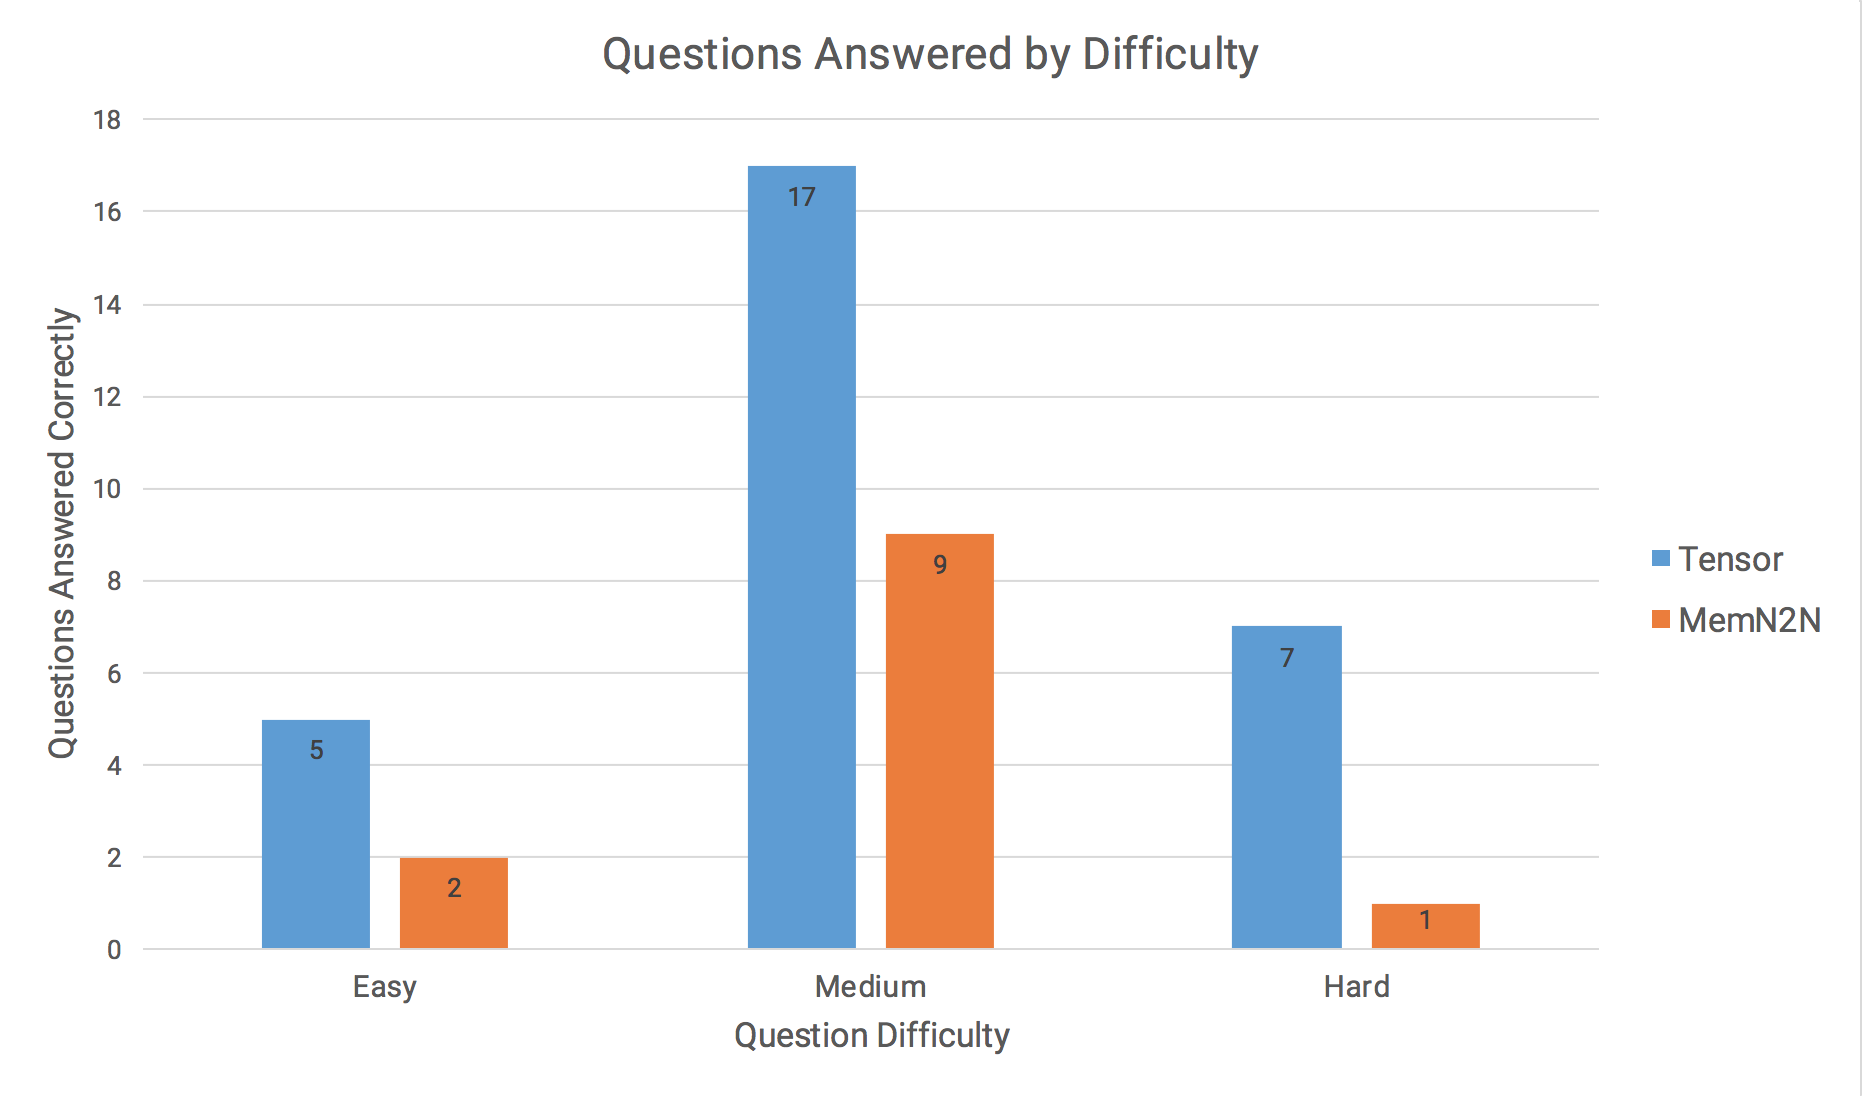
\includegraphics[width=0.7\textwidth,keepaspectratio]{figures/qa_by_difficulty.png}
    \caption{Total correct answers by difficulty level}
    \label{fig: qa_by_difficulty}
\end{figure}

\begin{figure}[!tb]
    \centering
    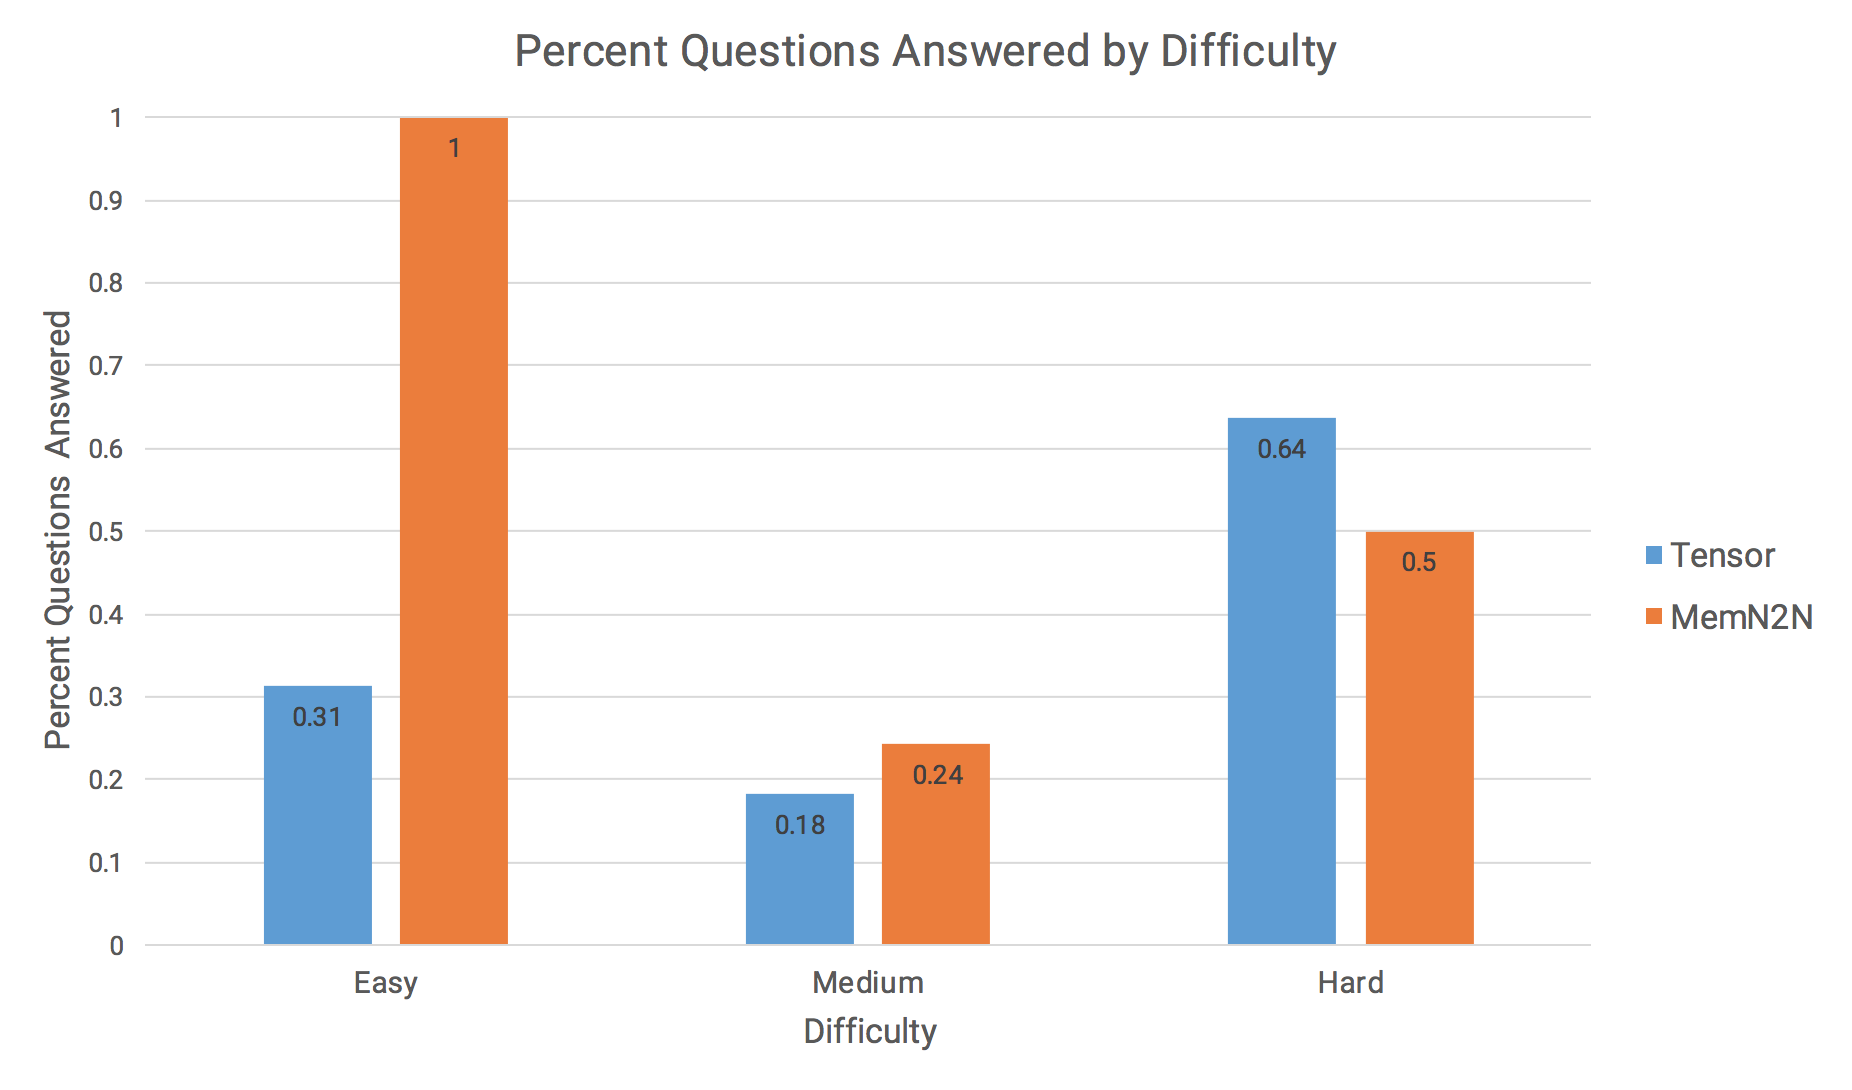
\includegraphics[width=0.7\textwidth,keepaspectratio]{figures/qa_by_difficulty_percent.png}
    \caption{Percent of questions of each difficulty level answered correctly}
    \label{fig: qa_by_difficulty_percent}
\end{figure}

The first observation we can make is that both models answer significantly more
Medium questions than Easy or Hard, but that their percentage on Medium
questions is lowest. This point is actually quite subtle. The full data tables
demonstrate that there are far more Medium questions in general than Easy or
Hard. However, the huge number of Medium questions means that the types of
Medium questions are also quite varied. Whether the percentage of Medium
questions answered correctly is so low is because there are simply far more
Medium questions or because there are types of Medium questions that both models
score poorly on (such as compare/contrast questions across passages) is unclear.

The second observation we make is that the MemN2N model scores perfectly on the
Easy questions and 50\% on the Hard questions. The problem with analyzing this
point is that the sample size is simply too small to make any claims about the
MemN2N's performance on Easy or Hard questions. We can definitively say that
the model was able to answer at least one of each type of question, even given
the limited test size, but we cannot claim more than that.

The third important observation here is that the tensor model answers a very
high percentage of Hard questions correctly. This is partially due to the
relatively small sample size (only 11), but also a consequence of the way in
which the tensor model is actually answering these questions. Consider Test 3
Section 2, where the tensor model answers 2 out of 4 Hard questions correctly.
This is actually another passage that contains two smaller passages, but both of
the Hard questions the model gets right deal with only one of the passages. In
fact, both questions ask about the meaning of a specific phrase in the context
of the passage. The tensor model is actually able to match the words in the
phrase with entities in the knowledge graph, and then match the answer choice
with the relevant information about the matched entity.

As far as questions go, these are actually some of the easiest for the tensor
model to answer because they do not require any high-level analysis. They simply
require matching words in the question to entities in the graph, and then
matching the corresponding graph element to words in the answer choice. This
is exactly how the tensor model works, by using word2vec to match words in the
question to entities in the graph, and then matching the relevant information to
words in the answer choices.

This analysis leads us to a key observation. The difficulty standards for humans
are not at all similar to the difficulty standards of our models. The Hard
questions described in the paragraph above can be very difficult for human
readers, because they require understanding the given phrase in context and then
translating it into one of the answer choices. Essentially, these questions
require fully understanding the phrase as well as its context. Our models,
however, do not need to fully understand the phrase or its context; they simply
need to match words in the question to entities in the graph. On the other hand,
questions marked Easy can be very difficult for our models (namely the tensor model,
as the MemN2N scored 2 / 2 on all its Easy questions). Some Easy questions ask
about the author's possible opinion on some topic that is not directly contained
in the text. For many humans these can be answered simply by understanding the
author's tone throughout the passage. Our models cannot understand tone, and
cannot process information not contained in the knowledge graph. These types
of questions are therefore impossible for them to answer.

\subsection{Comparing Tensor Model to MemN2N}
\label{Comparing Tensor Model to MemN2N}

Figure~\ref{fig: qa_by_test} shows the percent of questions answered correctly
by each model on each test. There are several striking observations. The first
is that the tensor model scores quite consistently, varying by just over 10\%
across all three tests. The MemN2N model is very volatile, in fact scoring the
single lowest and highest performances across both models and all tests.

\begin{figure}[!tb]
    \centering
    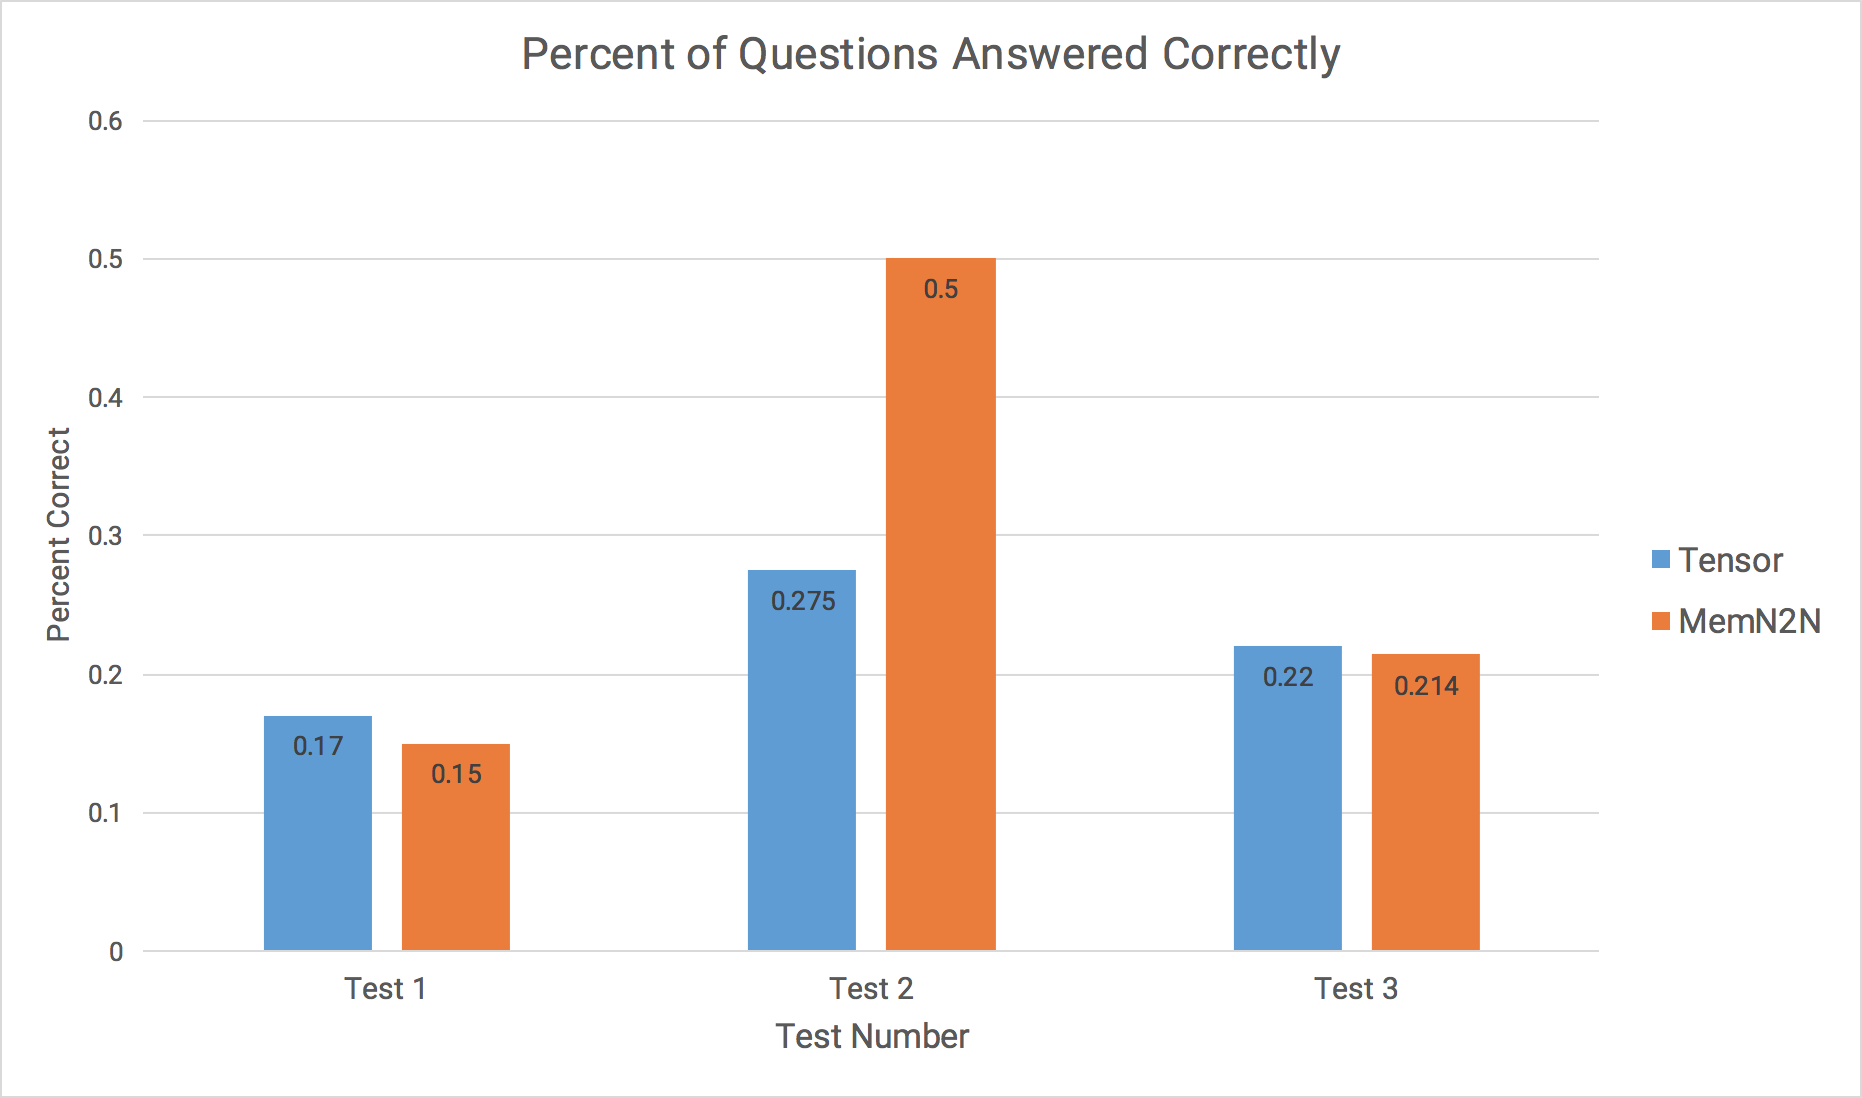
\includegraphics[width=0.7\textwidth,keepaspectratio]{figures/qa_by_test.png}
    \caption{Percent of questions on each test answered correctly}
    \label{fig: qa_by_test}
\end{figure}

This result is to be expected, as we discussed in Section \ref{Model Comparison}
how the tensor model is more mathematically sound while the neural net model
does not have as clear mathematics describing how it works. The MemN2N's
flexibility allowed it to score very high on Test 2, but at the same time score
very low on Test 1.

We also note that the models scored relatively similar on all of the tests. They
both scored lowest on Test 1, second-best on Test 3, and highest on Test 2.
Additionally, on both Test 1 and 3, the scores for the tensor and MemN2N are
almost identical, differing by no more than 2\%. This result is partially due to
the small sample size of MemN2N questions. Nevertheless, that the two models
have similar scores across all three tests indicates that for a given knowledge
graph they find the hidden representation of the knowledge graph equally well.
We conclude that the two models are, for the most part, equally viable. Across
the three tests, the tensor model scores barely higher than the MemN2N model on
Tests 1 and 3, but significantly worse on Test 2. The results demonstrate that
the tensor model is the better general choice, as it guarantees some amount of
competence, but at the same time it will not score very high. The MemN2N will
most likely score slightly worse than the tensor model, but has much higher
potential.

\section{Future Work}
\label{Future Work}

We hope this work is just the start of research into answering SAT questions and
tackling machine comprehension tasks of similar difficulty. To that end, we
present several ways to improve the models discussed in this paper. These
improvements fall in three major areas: linguistic analysis, tensor model, and
neural network.

\subsection{Linguistic Analysis}
\label{Linguistic Analysis}

There are three instances in our model where we need to analyze the semantic or
structural information of text. The first is extracting the knowledge graph
triples from the passage text. The second is parsing the question and
understanding what it is asking. The third is choosing an answer choice given
the information output by the model - this applies only to the tensor model.

\subsubsection{Knowledge Graph Extraction Improvements}
\label{Knowledge Graph Extraction Improvements}

There are some drawbacks to the way we currently extract the knowledge graph
triples from the text. Some information is lost in the extraction process.
Because the subject is forced to be $\text{entity}_1$ we lose information about
the direct object. For example, in the sentence in Figure~\ref{fig: dependency
extraction}, we learn that the dog likes sausage but not that the sausage is
spicy.

Additionally, SAT sentences are very difficult to parse. Most have multiple
clauses, and normally unusual structural elements such as the colon or dash are
quite commonplace. One sentence used in an actual passage is: \textit{The critic
Edumund Wilson was not a self-conscious letter writer or one who tried to
sustain studied mannerisms.} We are able to extract the triple $\langle
\text{Wilson}, \,\text{was}, \,\text{writer} \rangle$ but due to the complicated
structure of the sentence we are not able to extract that Wilson was not
self-conscious or that Wilson did not \textit{try to sustain studied
mannerisms.} Overall we can extract the most important points, but we often miss
the subtleties of the sentence.

If we can add more semantic rules to triple extraction then both the tensor
model as well as the MemN2N could have more information at hand to answer the
question. Right now we only focus on the \textit{nsubj} and \textit{dobj} or
\textit{cop} dependencies. One useful dependency we could add is the
\textit{amod} dependency, which is for adjectival modifiers \cite{De2014}. This
could help us capture descriptive information about entities that is not given
with a copular verb. We can also focus on entities that are not the nominal
subject, or add logic to handle sentences with multiple clauses.

\subsubsection{Question Parsing}
\label{Question Parsing}

In our existing model, we vectorize a given question by using word2vec to
calculate the similarity of every word in the sentence (excluding stopwords) to
every possible entity and relation, and choosing the 2 entities or entity and
relation that have highest similarity to question words. This works well when
the question tests a specific concept, but not when the question is more
complicated. This system runs into the same problem as bag-of-words matching,
where the semantic and structural information of the sentence is lost.

A better way to tackle question parsing would be to feed the questions through
the knowledge graph extraction program, and extract the information from the
question. However, because we need to frame the question as a query on the
knowledge graph we would modify the extraction program to extract triples with a
missing entity or relation. We can then try to fill in these missing elements
using the original knowledge graph, and match the resulting filled-in triples to
the answer choices. The answer would be the choice with strongest match.
Implementing this would require the improved deep extractor discussed above in
Section \ref{Knowledge Graph Extraction Improvements}.

\subsubsection{Choosing an Answer}
\label{Choosing an Answer}

Currently in the tensor model we choose an answer similarly to the way we parse
a question- by using word2vec to find the single word which matches the model's
output best. Often, the answer choices are sentences too, so we need to be able
to parse them. Just as with the questions we can feed the choices through the
Knowledge Graph extractor to find a set of triples. We then need to create some
metric to match triples and use it to pick the best choice.

\subsection{Tensor Model Improvements}
\label{Tensor Model Improvements}

There are several improvements that can be made to the tensor model. The first
is that the model's accuracy can be affected greatly by errors in the knowledge
graph extraction process. We need to find a way to make the tensor model robust
to such fluctuations. The best way to do this is to use an ensemble training
method. We can take the knowledge graph tensor and create several variants, each
slightly different from the original. Each of these are trained separately, and
then put together to create the actual approximation. This approximation has
several redundancies and is therefore less affected by errors in the original
knowledge graph. Ensemble learning methods are common in many machine learning
algorithms.

Another improvement that can be made to the tensor model is to provide
supervision in the training process. Because the model is not trained on the
actual questions, it cannot learn from the structure of the questions. By adding
a small supervised training component, we can achieve the flexibility of the
MemN2N while keeping the performance guarantee of the tensor model.

\subsection{MemN2N Improvements}
\label{MemN2N Improvements}

There are two main improvements we can make to the Memory Network. The first is
with the underlying architecture itself. The input vectors must be embedded with
matrices $A,C$. Since each passage has a tensor of different shape, we cannot
reuse $A,C$ across passages. We discussed in Section \ref{Evaluation Process}
how it is advantageous to train on just one passage at a time. However, with the
neural network there may be some underlying patterns across passages that we are
not able to capture currently. If the dimensionality constraints on the
architecture are loosened, the MemN2N model can be trained across passages and
even across tests. This means that the model could be trained on one particular
test, and run fully on another test.

The second possibility is to improve the model's consistency while preserving
its flexibility. The biggest drawback of the MemN2N currently is that it
occasionally has very poor performance. If we can train the model such that it
will be able to answer certain types of questions with high probability then the
model will be more reliable. For example, the tensor model is able to answer
most questions that ask for the meaning of some phrase in context (Section
\ref{Performance by Difficulty}). If the model is more reliable and consistent
while still flexible, then it can become the best tool for machine
comprehension. The very nature of neural network training makes it hard to
create consistency, but if the MemN2N has the ability to train across tests then
a large training corpus can help it achieve the desired consistency.

\section{Conclusion}
\label{Conclusion}

In this work we present an approach to machine comprehension tasks that uses
semantic and structural information instead of simple word-matching. We discuss
how any text can be represented as a knowledge graph of entity-relation triples
and questions about the text can be converted into queries on the graph. These
queries can be answered with either link prediction or entity prediction. We use
the Stanford NLP Toolkit's Dependency Parser \cite{Manning2014, Chen2014} to
turn every sentence in the text into a dependency graph, and then use semantic
rules to extract the information in triple form and create the knowledge graph.
We present two methods to answer the knowledge graph queries. We first present a
tensor decomposition approach, which factorizes the knowledge graph into a
product of matrices representing the latent properties of the graph. We improve
the RESCAL \cite{Nickel2011, Chang2014} method to use Semantically Smooth
Embedding \cite{Guo2015}. The second approach uses neural networks. We enhance
the Memory Networks \cite{Weston2015a, Sukhbaatar2015} architecture and
generalize it so that it can take any arbitrary knowledge graph and question
as input.

We evaluate the tensor decomposition and Memory Networks methods on three full
SAT reading comprehension tests. We demonstrate that the methods are able to
answer questions correctly using the actual semantic and structural meaning of
the original text. We also prove that our enhanced models perform better than
their respective baselines. The tensor decomposition model mostly outperforms
the Memory Networks model, but the Memory Networks model has a higher potential
to perform well. We discuss the types of questions which are possible for these
models to answer and which require a higher level of analysis. Finally, we
present possible extensions to our models. These include stronger semantic
parsing, making the tensor model more robust, and improving the Memory Network's
consistency.

The main goal of this research was to create a general model that could be used
to tackle a machine comprehension task that is much harder than the standard
MCTest \cite{Richardson2013} and bAbi \cite{Weston2015} datasets. We wanted to
show that these models could actually capture the semantic and structural
information of the text, and use that to answer questions. In this regard we
have definitely succeeded. Both models are able to parse the meaning of the text
as well as the questions, and use that information to find the correct answers.
There is still much room for improvement, however. We hope that the ideas
presented here will be useful in further machine comprehension research.

\newpage
\bstctlcite{bstctl:etal, bstctl:nodash, bstctl:simpurl}
\bibliographystyle{IEEEtranS}
\bibliography{final_references}
\newpage

\section{Appendix}
\label{Appendix}

\subsection{Derivation of Output Layer Error}
\label{Derivation of Output Layer Error}

In this section we present the derivation for the error of an output node of an
RNN with cross-entropy loss and softmax at the output layer. Softmax and
cross-entropy loss $C$ are defined in Section \ref{Recurrent Neural Networks}.
The Let us consider an output layer with $n$ nodes. Define $z_i$ as the quantity
before activation function at the output layer, and $\hat{y}_i$ as the final
output of node $i$. The true output of node $i$ is $y_i$. The output vectors can
be written as $\mathbf{\hat{y}},\,\mathbf{y}$. Note that $y$ is a one-hot
vector, so exactly one $y_i = 1$ and all other $y_j = 0$. The output node error
is calculated as $\dfrac{\partial C}{\partial z_i}$.

\begin{equation}
    \label{eq: output layer value}
    \hat{y}_i = \text{Softmax}(z_i) = \dfrac{e^{z_i}}{\sum\limits_{j=1}^n e^{z_j}} = \dfrac{e^{z_i}}
    {e^{z_i} + \sum\limits_{j\neq i} e^{z_j}}
\end{equation}

The partial derivatives yield

\begin{equation}
    \label{eq: output partials}
    % \begin{gather*}
    \begin{aligned}
        \dfrac{\partial \hat{y}_i}{\partial z_i} &= \dfrac{\sum\limits_{j=1}^n e^{z_j}(e^{z_i}) - e^{z_i}(e^{z_i})}
        {\left( \sum\limits_{j=1}^n e^{z_j} \right)^2}
        = \dfrac{e^{z_i}\sum\limits_{j=1}^n e^{z_j}}{\left( \sum\limits_{j=1}^n e^{z_j} \right)^2}
        - \left( \dfrac{e^{z_i}}{ \sum\limits_{j=1}^n e^{z_j} } \right)^2 \\
        &\phantom{=} \\
        &= \hat{y}_i - \hat{y}_i^2
        = \hat{y}_i\left( 1 - h_i \right) \\
        &\phantom{=} \\
        \dfrac{\partial \hat{y}_i}{\partial z_j} &= \dfrac{\sum\limits_{j=1}^n e^{z_j}(0) - e^{z_i}(e^{z_i})}
        {\left( \sum\limits_{j=1}^n e^{z_j} \right)^2}
        = \dfrac{-e^{z_i}}{\sum\limits_{j=1}^n e^{z_j}}\dfrac{e^{z_j}}{\sum\limits_{j=1}^n e^{z_j}} \\
        &\phantom{=} \\
        &= -\hat{y}_i\hat{y}_j
    \end{aligned}
    % \end{gather*}
\end{equation}

When we take the partial of $C$ with respect to the individual $z_i$, we need
$\dfrac{\partial \hat{y}_i}{\partial z_i}$ as well as $\dfrac{\partial
\hat{y}_j}{\partial z_i}$.

$$
\dfrac{\partial \hat{y}_i}{\partial z_j} =
\begin{cases}
    \hat{y}_i(1-\hat{y}_i) & \text{if } i = j \\
    -\hat{y}_i\hat{y}_j & \text{if } i \neq j
\end{cases}
$$

Now we derive the output node error using the results of Equation~\eqref{eq: output partials}.
\begin{equation}
    \label{eq: loss function partial to h}
    \begin{aligned}
        \dfrac{\partial C}{\partial \hat{y}_i} &= -\dfrac{y_i}{\hat{y}_i} \\
        &\phantom{=} \\
        % \dfrac{\partial C}{\partial z_i} &= \dfrac{\partial C}{\partial h_i}
        \dfrac{\partial C}{\partial z_i} &= \sum\limits_{j=1}^n \dfrac{\partial C}{\partial \hat{y}_j}\dfrac{\partial \hat{y}_j}{\partial z_i} =
            \dfrac{\partial C}{\partial \hat{y}_i}\dfrac{\partial \hat{y}_i}{\partial z_i} + \sum\limits_{j\neq i} \dfrac{\partial C}{\partial \hat{y}_j}\dfrac{\partial \hat{y}_j}{\partial z_i} \\
        &\phantom{=} \\
        \dfrac{\partial C}{\partial \hat{y}_i}\dfrac{\partial \hat{y}_i}{\partial z_i} &= -\dfrac{y_i}{\hat{y}_i} \hat{y}_i (1-\hat{y}_i) = -y_i(1-\hat{y}_i) \\
        &\phantom{=} \\
        \dfrac{\partial C}{\partial \hat{y}_j}\dfrac{\partial \hat{y}_j}{\partial z_i} &= -\dfrac{y_j}{\hat{y}_j} \left(-\hat{y}_i\hat{y}_j\right) = y_j\hat{y}_i
    \end{aligned}
\end{equation}

Summing together these partials yields
\begin{equation}
    \dfrac{\partial C}{\partial z_i} = -y_i(1-\hat{y}_i) + \sum\limits_{j\neq i} y_j\hat{y}_i =
        -y_i + y_i\hat{y}_i + \sum\limits_{j\neq i} y_j\hat{y}_i = -y_i + \sum\limits_{j = 1}^n y_j\hat{y}_i = -y_i + \hat{y}_i\sum\limits_{j=1}^n y_j
\end{equation}

However, we know that $\sum_{j=1}^n y_j = 1$ because $\mathbf{y}$ is a one-hot vector. This
yields our desired result.
\begin{equation}
    \dfrac{\partial C}{\partial z_i} = \hat{y}_i - y_i
\end{equation}

This is a very useful result. It can be calculated very easily and in parallel
for each node, which prevents backpropagation from becoming a bottleneck and
allows the RNN to learn quickly.

% When we have $n$ output nodes, our cost function is $\sum^n_i y_i
% \log(\hat{y_i})$. Consider some output
\subsection{Full Evaluation Data}
\label{Full Evaluation Data}
Here we present the full evaluation data on three practice tests.

% Please add the following required packages to your document preamble:
% \usepackage{booktabs}
\begin{table}[b]
\scriptsize
\centering
\caption{Evaluation on Test 1}
\label{tab: Evaluation on Test 1}
% \begin{tabularx}{\textwidth}{XXXXXXXXXX}
\begin{tabularx}{\textwidth}{lXXXXXXX}
\toprule
                         & \textbf{Number} & \textbf{Difficulty} & \textbf{Correct\newline Answer} & \textbf{Tensor\newline w/o Reg} & \textbf{Tensor\newline w/ Reg} & \textbf{1-layer\newline MemN2N} & \textbf{3-layer\newline MemN2N} \\ \midrule
\textbi{Section 1}       &            &   &       &                         &                        &                         &                             \\ \midrule
\textbf{Small}           & 9          & E & E     & A                       & A                      & -                       & -                           \\
\textbf{}                & 10         & M & B     & A                       & D                      & -                       & -                           \\
\textbf{}                & 11         & E & D     & \g{D}                   & \g{D}                   & -                       & -                           \\
\textbf{}                & 12         & E & D     & E                       & E                      & -                       & -                           \\
\textbf{Long}            & 13         & M & E     & C                       & D                      & train                   & train                       \\
\textbf{}                & 14         & E & D     & \g{D}                   & \g{D}                      & train                   & train                       \\
\textbf{}                & 15         & M & B     & E                       & \g{B}                      & train                   & train                       \\
\textbf{}                & 16         & H & A     & E                       & \g{A}                      & train                   & train                       \\
\textbf{}                & 17         & H & A     & \g{A}                   & \g{A}                      & train                   & train                       \\
\textbf{}                & 18         & E & C     & E                       & D                      & train                   & train                       \\
\textbf{}                & 19         & M & A     & D                       & D                      & train                   & train                       \\
\textbf{}                & 20         & M & B     & D                       & A                      & train                   & train                       \\
\textbf{}                & 21         & M & B     & E                       & E                      & A                       & A                           \\
\textbf{}                & 22         & M & C     & A                       & A                      & A                       & A                           \\
\textbf{}                & 23         & M & B     & D                       & D                      & A                       & A                           \\
\textbf{}                & 24         & E & A     & \g{A}                   & B                      & \g{A}                       & \g{A}                           \\ \midrule
\textbi{Section 2}       &            &   &       &                         &                        &                         &                             \\ \midrule
\textbf{Medium}          & 13         & M & C     & B                       & B                      & train                   & train                       \\
\textbf{}                & 14         & E & B     & C                       & D                      & train                   & train                       \\
\textbf{}                & 15         & M & C     & E                       & E                      & train                   & train                       \\
\textbf{}                & 16         & E & E     & B                       & B                      & train                   & train                       \\
\textbf{}                & 17         & E & D     & A                       & A                      & C                       & C                           \\
\textbf{}                & 18         & M & C     & A                       & A                      & \g{C}                       & D                           \\
\textbf{Medium}          & 19         & M & E     & B                       & \g{E}                  & train                   & train                       \\
\textbf{}                & 20         & E & C     & E                       & E                      & train                   & train                       \\
\textbf{}                & 21         & M & D     & \g{D}                   & B                      & train                   & train                       \\
\textbf{}                & 22         & M & E     & \g{E}                   & \g{E}                  & train                   & train                       \\
\textbf{}                & 23         & M & A     & D                       & E                      & E                       & C                           \\
\textbf{}                & 24         & M & B     & \g{B}                   & \g{B}                  & E                       & C                           \\ \midrule
\textbi{Section 3}       &            &   &       &                         &                        &                         &                             \\ \midrule
\textbf{Long}            & 7          & M & B     & A                       & A                      & train                   & train                       \\
\textbf{}                & 8          & M & A     & C                       & C                      & train                   & train                       \\
\textbf{}                & 9          & M & D     & E                       & E                      & train                   & train                       \\
\textbf{}                & 10         & M & E     & D                       & D                      & train                   & train                       \\
\textbf{}                & 11         & M & A     & B                       & B                      & train                   & train                       \\
\textbf{}                & 12         & E & A     & C                       & C                      & train                   & train                       \\
\textbf{}                & 13         & E & D     & E                       & B                      & train                   & train                       \\
\textbf{}                & 14         & M & D     & B                       & B                      & train                   & train                       \\
\textbf{}                & 15         & M & E     & A                       & A                      & D                       & D                           \\
\textbf{}                & 16         & M & E     & A                       & A                      & D                       & D                           \\
\textbf{}                & 17         & M & C     & D                       & D                      & D                       & D                           \\
\textbf{}                & 18         & M & A     & D                       & D                      & D                       & \g{A}                           \\
\textbf{}                & 19         & M & E     & C                       & C                      & D                       & D                           \\ \midrule
\textbf{Correct}         &            &   &       & 7                       & 8                      & 2                       & 2                           \\
\textbf{Questions}       &            &   &       & 41                      & 41                     & 13                      & 13                          \\ \bottomrule
\end{tabularx}
% \end{tabular}
\end{table}

% Please add the following required packages to your document preamble:
% \usepackage{booktabs}
\begin{table}[]
\footnotesize
\centering
\caption{Evaluation on Test 2}
\label{tab: Evaluation on Test 2}
\begin{tabular}{llllll}
\toprule
\multicolumn{1}{c}{}     & \multicolumn{1}{c}{\textbf{Number}} & \multicolumn{1}{c}{\textbf{Difficulty}} & \multicolumn{1}{c}{\textbf{Correct Answer}} & \multicolumn{1}{c}{\textbf{Tensor w/ Reg}} & \multicolumn{1}{c}{\textbf{3-layer MemN2N}} \\ \midrule
\textbi{Section 1}       &                                     &                                         &                                             &                                            &                                             \\ \midrule
\textbf{Long}            & 13                                  & M                                       & A                                           & C                                          & train                                       \\
\textbf{}                & 14                                  & M                                       & C                                           & A                                          & train                                       \\
\textbf{}                & 15                                  & M                                       & E                                           & D                                          & train                                       \\
\textbf{}                & 16                                  & M                                       & D                                           & \g{D}                                      & train                                       \\
\textbf{}                & 17                                  & M                                       & D                                           & B                                          & train                                       \\
\textbf{}                & 18                                  & M                                       & D                                           & E                                          & train                                       \\
\textbf{}                & 19                                  & M                                       & E                                           & \g{E}                                      & train                                       \\
\textbf{}                & 20                                  & M                                       & C                                           & A                                          & train                                       \\
\textbf{}                & 21                                  & M                                       & A                                           & B                                          & E                                           \\
\textbf{}                & 22                                  & M                                       & B                                           & A                                          & \g{B}                                           \\
\textbf{}                & 23                                  & H                                       & B                                           & \g{B}                                      & \g{B}                                           \\
\textbf{}                & 24                                  & M                                       & A                                           & B                                          & D                                           \\ \midrule
\textbi{Section 2}       &                                     &                                         &                                             &                                            &                                             \\ \midrule
\textbf{Medium}          & 10                                  & M                                       & A                                           & B                                          & train                                       \\
\textbf{}                & 11                                  & M                                       & A                                           & B                                          & train                                       \\
\textbf{}                & 12                                  & M                                       & D                                           & A                                          & train                                       \\
\textbf{}                & 13                                  & E                                       & C                                           & \g{C}                                      & train                                       \\
\textbf{}                & 14                                  & M                                       & B                                           & \g{B}                                      & D                                           \\
\textbf{}                & 15                                  & M                                       & A                                           & E                                          & \g{A}                                           \\
\textbf{Medium}          & 16                                  & M                                       & E                                           & A                                          & train                                       \\
\textbf{}                & 17                                  & E                                       & D                                           & B                                          & train                                       \\
\textbf{}                & 18                                  & E                                       & A                                           & \g{A}                                          & train                                       \\
\textbf{}                & 19                                  & M                                       & C                                           & E                                          & train                                       \\
\textbf{}                & 20                                  & H                                       & E                                           & B                                          & train                                       \\
\textbf{}                & 21                                  & M                                       & A                                           & \g{A}                                          & train                                       \\
\textbf{}                & 22                                  & M                                       & C                                           & \g{C}                                          & E                                           \\
\textbf{}                & 23                                  & M                                       & B                                           & E                                          & E                                           \\
\textbf{}                & 24                                  & M                                       & B                                           & \g{B}                                          & E                                           \\ \midrule
\textbi{Section 3}       &                                     &                                         &                                             &                                            &                                             \\ \midrule
\textbf{Long}            & 7                                   & M                                       & B                                           & C                                          & train                                       \\
\textbf{}                & 8                                   & E                                       & B                                           & E                                          & train                                       \\
\textbf{}                & 9                                   & M                                       & D                                           & A                                          & train                                       \\
\textbf{}                & 10                                  & M                                       & D                                           & C                                          & train                                       \\
\textbf{}                & 11                                  & E                                       & C                                           & E                                          & train                                       \\
\textbf{}                & 12                                  & M                                       & A                                           & E                                          & train                                       \\
\textbf{}                & 13                                  & M                                       & B                                           & A                                          & train                                       \\
\textbf{}                & 14                                  & H                                       & E                                           & \g{E}                                      & train                                       \\
\textbf{}                & 15                                  & M                                       & B                                           & A                                          & \g{B}                                           \\
\textbf{}                & 16                                  & M                                       & E                                           & \g{E}                                      & \g{E}                                           \\
\textbf{}                & 17                                  & M                                       & D                                           & C                                          & \g{D}                                           \\
\textbf{}                & 18                                  & M                                       & B                                           & A                                          & \g{B}                                           \\
\textbf{}                & 19                                  & M                                       & A                                           & C                                          & C                                           \\ \midrule
\textbf{Correct}         &                                     &                                         &                                             & 11                                         & 7                                           \\
\textbf{Questions}       &                                     &                                         &                                             & 40                                         & 14                                          \\ \bottomrule
\end{tabular}
\end{table}

% Please add the following required packages to your document preamble:
% \usepackage{booktabs}
\begin{table}[]
\footnotesize
\centering
\caption{Evaluation on Test 3}
\label{tab: Evaluation on Test 3}
\begin{tabular}{@{}llllll@{}}
\toprule
\multicolumn{1}{c}{}    & \multicolumn{1}{c}{\textbf{Number}} & \multicolumn{1}{c}{\textbf{Difficulty}} & \multicolumn{1}{c}{\textbf{Correct Answer}} & \multicolumn{1}{c}{\textbf{Tensor w/ Reg}} & \multicolumn{1}{c}{\textbf{3-layer MemN2N}} \\ \midrule
\textbi{Section 1}      &                                     &                                         &    &    &                                             \\ \midrule
\textbf{Medium}         & 10                                  & E                                       & B  & C  & train                                       \\
\textbf{}               & 11                                  & M                                       & C  & E  & train                                       \\
\textbf{}               & 12                                  & E                                       & A  & B  & train                                       \\
\textbf{}               & 13                                  & M                                       & D  & A  & train                                       \\
\textbf{}               & 14                                  & M                                       & C  & A  & \g{C}                                           \\
\textbf{}               & 15                                  & E                                       & D  & C  & C                                           \\
\textbf{Medium}         & 16                                  & M                                       & A  & \g{A}  & train                                       \\
\textbf{}               & 17                                  & H                                       & B  & A  & train                                       \\
\textbf{}               & 18                                  & M                                       & E  & B  & train                                       \\
\textbf{}               & 19                                  & M                                       & D  & A  & train                                       \\
\textbf{}               & 20                                  & M                                       & D  & B  & train                                       \\
\textbf{}               & 21                                  & M                                       & D  & C  & train                                       \\
\textbf{}               & 22                                  & M                                       & A  & A  & E                                           \\
\textbf{}               & 23                                  & E                                       & E  & \g{E}  & \g{E}                                           \\
\textbf{}               & 24                                  & M                                       & B  & C  & E                                           \\ \midrule
\textbi{Section 2}      &                                     &                                         &    &    &                                             \\ \midrule
\textbf{Long}           & 13                                  & M                                       & E  & A  & train                                       \\
\textbf{}               & 14                                  & M                                       & C  & E  & train                                       \\
\textbf{}               & 15                                  & M                                       & D  & A  & train                                       \\
\textbf{}               & 16                                  & H                                       & D  & \g{D}  & train                                       \\
\textbf{}               & 17                                  & M                                       & B  & A  & train                                       \\
\textbf{}               & 18                                  & M                                       & C  & \g{C}  & train                                       \\
\textbf{}               & 19                                  & H                                       & B  & \g{B}  & train                                       \\
\textbf{}               & 20                                  & M                                       & B  & E  & train                                       \\
\textbf{}               & 21                                  & H                                       & D  & B  & B                                           \\
\textbf{}               & 22                                  & H                                       & E  & A  & B                                           \\
\textbf{}               & 23                                  & M                                       & A  & \g{A}  & E                                           \\
\textbf{}               & 24                                  & M                                       & E  & D  & A                                           \\ \midrule
\textbi{Section 3}      &                                     &                                         &    &    &                                             \\ \midrule
\textbf{Long}           & 7                                   & E                                       & D  & B  & train                                       \\
\textbf{}               & 8                                   & M                                       & E  & \g{E}  & train                                       \\
\textbf{}               & 9                                   & M                                       & D  & B  & train                                       \\
\textbf{}               & 10                                  & M                                       & D  & A  & train                                       \\
\textbf{}               & 11                                  & M                                       & B  & A  & train                                       \\
\textbf{}               & 12                                  & E                                       & C  & E  & train                                       \\
\textbf{}               & 13                                  & M                                       & A  & \g{A}  & train                                       \\
\textbf{}               & 14                                  & M                                       & E  & D  & train                                       \\
\textbf{}               & 15                                  & M                                       & C  & A  & E                                           \\
\textbf{}               & 16                                  & M                                       & B  & D  & B                                           \\
\textbf{}               & 17                                  & M                                       & E  & C  & D                                           \\
\textbf{}               & 18                                  & M                                       & A  & B  & D                                           \\
\textbf{}               & 19                                  & M                                       & D  & E  & \g{D}                                           \\ \midrule
\textbf{Correct}        &                                     &                                         &    & 9  & 3                                           \\
\textbf{Questions}      &                                     &                                         &    & 41 & 14                                          \\ \bottomrule
\end{tabular}
\end{table}

\end{document}
